\documentclass[11pt,twoside,slovak,a4paper]{article}

\usepackage[slovak]{babel}
\usepackage[T1]{fontenc}
\usepackage[utf8]{inputenc}
\PassOptionsToPackage{hyphens}{url}
\usepackage{mathptmx}
%\usepackage[IL2]{fontenc}
\usepackage{babel}
\usepackage{helvet}
\usepackage[scaled]{uarial}
\usepackage[utf8]{inputenc}
\usepackage[nottoc]{tocbibind}
\usepackage{fancyhdr}
\usepackage{ifthen}
\usepackage{listings}
\usepackage{graphicx}
\usepackage{titlesec}
%\usepackage{url} % príkaz \url na formátovanie URL
\usepackage{hyperref} % odkazy v texte budú aktívne (pri niektorých triedach dokumentov spôsobuje posun textu)
\hypersetup{
	hidelinks = true
}
\raggedbottom

\usepackage{cite}
\usepackage{times}
\usepackage{comment}

\usepackage[dvips,dvipdfm,a4paper,centering,textwidth=14cm,top=4.6cm,headsep=.6cm,footnotesep=1cm,footskip=0.6cm,bottom=3.8cm]{geometry}
\usepackage{amsmath}
\usepackage{graphicx}

\usepackage{etoolbox}
\linespread{1.5}

\pagestyle{myheadings}

\begin{document}
	
	\begin{titlepage}
		\centering
		\newlength{\myind}
		\addtolength{\myind}{57mm}
		
		\newlength{\myrulelength}
		%\addtolength{\myrulelength}{.6\marginparwidth}
		\addtolength{\myrulelength}{\textwidth}
		\newcommand{\myrule}{\parbox{\myrulelength}{\hrulefill}}
		%\newcommand{\mybox}[1]{\hspace{.5\marginparwidth}\parbox{\myrulelength}{#1}}
		%\newcommand{\mycbox}[1]{\hspace{.5\marginparwidth}\parbox{\myrulelength}{\centering #1}}
		\newcommand{\mybox}[1]{\parbox{\myrulelength}{#1}}
		\newcommand{\mycbox}[1]{\parbox{\myrulelength}{\centering #1}}
		
		\begin{center}
			\large 		Slovenská technická univerzita v Bratislave\\
			Fakulta informatiky a informačných technológií	
			%\hrulefill		
		\end{center}

		
	%	\vspace{4mm}
		\myrule
		
		\begin{center}
			FIIT-5212-71998
		\end{center}
		
		\vspace{40mm}
		
		\mycbox{Peter Beňuš}
		
		\vspace{10mm}
		
		\mycbox{\LARGE \textbf{ \MakeUppercase {Automatické testovanie softvéru}}}
		
		\vspace{4mm}
		\mycbox{\large Bakalársky práca}
		
		
		\vfill
		\begin{flushleft}
			Študijný program: Informatika\\
			Študijný odbor: 9.2.1 Informatika\\
			Miesto vypracovania: Ústav informatiky, informačných systémov a softvérového inžinierstva, FIIT STU v Bratislave\\
			Vedúci bakalárskeho projektu: Ing. Karol Rástočný\\
			máj 2016
		\end{flushleft}
	\end{titlepage}
	
	
	\begin{titlepage}
		\begin{center}
			\large 		Slovenská technická univerzita v Bratislave\\
			\textbf{\MakeUppercase{Fakulta informatiky a informačných technológií}}\\
			\hrulefill
		\end{center}
		%\fontsize{14}{17}\MakeUppercase{\textbf{Automatické testovanie softvéru}}\\
		%\\
			\section*{Anotácia}
		Študijný program: Informatika\\
		Autor: Peter Beňuš\\
		Názov bakalárskej práce: Automatické testovanie softvéru \\
		Vedúci bakalárskej práce: Ing. Karol Rástočný\\
		máj 2016\\
		Práca sa venuje jednotkovému testovaniu softvéru. Obsahuje analýzu vlastností jednotkového testovania, z ktorých vyplývajú požiadavky na pracovné rámce určené na jednotkové testovanie. Na základe vlastností jednotkového testovania sme odvodili vlastnosti ideálneho testovacieho pracovného rámca na jednotkové testovanie. Vybraných je niekoľko pracovných rámcov pre jazyk C\# a Java patriacich do skupiny xUnit. Tieto pracovné rámce boli analyzované a pre jazyk Java aj experimentálne porovnané na prototype, ktorý riešil matematické úlohy. Každý pracovný rámec prináša zo sebou výhody aj nevýhody oproti ostatným. Porovnaním vlastností pracovných rámcov sme určili ich vhodnosť pre špecifické softvérové projekty.
	\end{titlepage}
	
	\begin{titlepage}
		\begin{center}
			\large 		Slovak University of Technology Bratislava\\
			\textbf{\MakeUppercase{Faculty of Informatics and Information Technologies}}\\
			\hrulefill
		\end{center}
		\section*{Annotation}
		Degree Course: Informatics\\
		Author: Peter Beňuš \\
		Title of bachelor thesis: Automatic Software Testing\\
		Supervisor: Ing. Karol Rástočný \\
		may 2016 \\
		Thesis is concerned with unit testing. In includes analysis of unit testing characteristics, from which follows requirements of unit testing frameworks. We derived characteristics of ideal unit test framework from it. Some of unit test frameworks, for C\# and Java belonging to xUnit group, was chosen. These framework was analysed and for Java they was also experimentaly tested on prototype of program, which solve mathematical problems. Every framework has advantages and disadvantages in comparison with others. We did comparison of unit testing frameworks characteristics and determine suitability of them for specific software projects.		
		
	\end{titlepage}
	
	\begin{titlepage}
		\tableofcontents
	\end{titlepage}
	
	
	\pagestyle{fancy}
	\fancyhf{}
	\fancyhead[RE,RO]{\thechapter \leftmark}
	\fancyfoot[CE,CO]{\thepage}
	\headheight 14pt
	\setcounter{page}{1}
	
	\thispagestyle{plain}
	\section{Úvod}
	Testovanie softvéru v súčastnosti naberá na dôležitosti a prikladá sa mu čoraz väčšia váha počas tvorby softvéru. Napriek tomu, že pri súčasnej komplexnosti rôznych programov nedokážeme zabezpečiť úplnú absenciu chýb má veľký význam sa snažiť tieto chyby minimalizovať.
	
	Testovanie môže prebiehať (a často aj prebieha) počas celej doby životného cyklu programu. Čím skôr je chyba odhalená a opravená tým menšie negatívne následky bude mať na výsledný produkt. Preto je dôležité testovať softvér od začiatku tvorby, od najmenších jednotiek, cez integráciu viacerých jednotiek a komponentov až po celé systémy, ktoré môžu byť zložené z viacerých programov.
	
	Medzi pracovnými rámcami nie sú porovnania vo vlastnostiach, ale zväčša len každý obhajuje svoj obľúbený pracovný rámec a preto sme sa rozhodli porovnať viacero pracovných rámcov na jednotkové testovanie a vytvoriť ich porovnanie čo najobjektívnejšie a nezohľadňovať len subjektívne pocity, ktoré vznikajú pri práci s každým pracovným rámcom.
		
	Tak ako sa v rôznych častiach životného cyklu softvéru testujú rôzne aspekty produktu, používajú sa aj rôzne prístupy testovania a softvér testujú rôzny ľudia. Jednotkové testovanie vykonávajú typicky programátori a testujú jednotlivé jednotky nezávisle od seba. Integračné a systémové testovanie majú na starosti testeri a ich úlohou je odhaliť chyby v komunikácií medzi komponentami, resp. programom a konkrétnym systémom. Akceptačné testovanie vykonáva už objednávateľ alebo cieľová skupina používateľov a jeho výsledkom je akceptovanie výsledného produktu, resp. neakceptovanie a nutnosť opravy\cite{Myers}.
	
	Jednotkové testovanie je typ testovania, ktorým sa musel zaoberať každý, kto už niečo programoval, pretože vždy začíname tým  vytvorením jednotky programu a postupne sa k tomu pridávajú ďaľšie. Dokonca je tento postup úplne nezávislý od toho či sa iba učíme programovať alebo už programovať vieme a vytvárame program na konkrétny účel. Výrazný rozdiel, ale môže byť v tom, že začiatočníci budú testovať svoje jednotky programu opakovaným spúšťaním, zadávaním rôznych vstupov a sledovaním výsledkov, ale skúsený programátor použije nejaký pracovný rámec, ktorý dokáže otestovať to čo treba za neho a upozorniť ho keď sa niekde nájde chyba.
	
	Pracovný rámec, ktorý by dokázal automaticky vykonávať jednotkové testovanie by bol preto veľkým prínosom pre programátorov, pretože by im zrýchlil a zjednodušil prácu. Preto sa snažíme nájsť pracovný rámec, ktorý dokáže prácu programátorom čo najviac zjednodušiť a zautomatizovať testovanie.
	
	V druhej a tretej kapitole dokumentu sa venujeme teoretickým vlastnostiam testovania softvéru a kľúčovým vlastnostiam jednotkového testovania. Poznatky z týchto kapitol nám umožnili vytvoriť spôsob hodnotenia pracovných rámcov, tak aby sme ich vedeli porovnať podľa ich skutočných vlastností. Tento spôsob hodnotenia je v štvrtej kapitole.
	
	V piatej kapitole opisujeme pracovné rámce na jednotkové testovanie pre jazyky C\# a Java. Kapitola obsahuje aj popis vlastností skupiny xUnit, do ktorej všetky tieto pracovné rámce patria.
	
	Kapitoly 6, 7 a 8 sú venované metóde testovania, hodnotenia a ich porovnania. Vychádzali sme s informácií získaných počas experimentálneho testovania pracovných rámcov na prototype vykonávajúcom matematické výpočty. Rámce sú zoradené podľa vhodnosti použitia, ale uvádzame aj ich vhodnosť na rôzne typy projektov, pretože najvhodnejší pracovný rámec na jeden typ projektu nemusí byť rovnako vhodný na všetky.	
	
	\newpage
	\thispagestyle{plain}
	\section{Testovanie softvéru}
	Testovanie softvéru je empirická činnosť, ktorá skúma kvalitu testovaného softvérového produktu vykonávaná na podanie informácií o kvalite všetkým zainteresovaným osobám\cite{Kaner2006}. V súčastnosti existuje veľa spôsobov testovania a veľa častí životného cyklu softvéru, v ktorých sa aplikujú iné typy testov. Testovanie softvéru môžeme rozdeliť na kategórie podľa postupu, ktorý sa používa pri testovaní, podľa spôsobu testovania a podľa úrovne testu.
	
	\subsection{Podľa postupu testovania}
		\subsubsection{Testovanie formou čiernej skrinky} 
			Testuje funkcionalitu bez informácií o tom ako je softvér implementovaný. Tester dostane iba informácie o tom, aký by mal byť výsledok testu po zadaní vstupných dát a kontroluje výstup softvéru či sú výstupné dáta totožné s očakávanými\cite{EST2002}. Test je konštruovaný z funkcionálnych vlastností, ktoré sú špecifikované požiadavkách na program\cite{Moha1991}.  Výhodou tohto typu testovania je, že tester nie je ovplyvnený štruktúrou zdrojového kódu a tým môže odhaliť chyby aj tam, kde to programátor nehľadal lebo to považoval za správne pri pohľade na zdrojový kód, ale bola tam chyba, ktorá zo zdrojového kódu nemusí byť viditeľná (napríklad nesprávne, resp. nedostatočné ošetrenie nekorektných vstupov). Hlavnou výhodou je, že tester nemusí poznať zdrojový kód a preto môže oveľa rýchlejšie vytvoriť testy. Nevýhodou je úroveň otestovania systému, pretože tvorca testov nevie ako program funguje, a preto veľmi pravdepodobne nebude schopný vytvoriť test, ktorý by testoval všetky vetvy programu. Používa sa pri jednotkovom, integračnom, systémovom a akceptačnom testovaní. Okrem použitia pri rôznych úrovniach testov sa využíva aj na validáciu softvéru\cite{EST2002}.
		\subsubsection{Testovanie formou bielej skrinky} 
			Pri tomto spôsobe testovania je testerovi známa vnútorná štruktúra softvéru a aj konkrétna implementácia. Test sa tvorí tak, aby bola otestovaná každá vetva zdrojového kódu\cite{EST2002}. Používa sa pri jednotkovom testovaní na skoré odhalenie čo najväčšieho množstva chýb, pri integračnom testovaní na testovanie správnej spolupráce rôznych jednotiek programu a aj pri regresnom testovaní, kde sa používajú recyklované testovacie prípady z integračného a jednotkového testovania a taktiež slúži na verifikáciu. Výhodou je schopnosť otestovať komplexne všetky vetvy, ktoré program na danej úrovni testu vykonáva, ale nevýhodou je, že tester musí mať dobré vedomosti o zdrojovom kóde a v niektorých prípadoch tvorenia testov môže byť znalosť zdrojového kódu nevýhoda, pretože sa tým nájdu len chyby v zdrojovom kóde, ale ťažko by sa odhaľovali chyby v prípadoch, na ktoré autor kódu nemyslel.
		\subsubsection{Testovanie formou sivej skrinky} 
			Spôsob testovania, pri ktorom je známy zdrojový kód (nemusí byť sprístupnený úplne celý), ale testy sa vykonávajú rovnako ako pri testovaní formou čiernej skrinky. Používa sa napríklad pri integračnom testovaní ak máme dva moduly od rôznych vývojárov a odkryté sú len rozhrania \cite{EST2002}. Poskytuje výhody obidvoch predchádzajúcich prístupov, ale má oproti nim aj nejaké nevýhody. Oproti testovaniu čiernou skrinkou má výhodu v lepšom pokrytí rôznych vetiev zdrojového kódu, ale je časovo náročnejšie na tvorbu testov. Oproti testovaniu bielou skrinkou je menej náročné na znalosť zdrojového kódu, pretože ho nemá prístupný celý, ale nepokrýva všetky vetvy programu a preto je menej komplexné.
	
	\subsection{Podľa spôsobu testovania}
		\subsubsection{Statické testovanie}
			Statické testovanie je často implicitné. Zahŕňa napríklad kontrolu zdrojového kódu programátorom jeho čítaním hneď po napísaní, kontrolu štruktúry a syntaxe kódu nástrojom alebo editorom, v ktorom sa zdrojový kód píše. Program nie je potrebné spúšťať, ale analýza zdrojového kódu založená na upravovacích pravidlách zistí v zdrojovom kóde rôzne možné chyby, ktoré sa zvyčajne objavujú v spravovaní pamäte, neinicializovaných premenných, výnimke nulového smerníku, porušení prístupu k poľu a taktiež pretečení vyrovnávacej pamäti\cite{Wei2014}.
			
			Veľmi dôležitou súčasťou statického testovania je posudzovanie zdrojového kódu (angl. codereview). Je to posudzovanie zdrojového kódu iným vývojárom za účelom dosiahnutia čo najvyššej kvality. Formálny variant tohto posudzovania bol veľmi dlho efektívnym kvalitatívnym prínosom pri tvorbe softvéru, ale za relatívne vysokú cenu. Preto sa v poslednej dobe začala používať odľahčené a neformálne posudzovanie založené na nástrojoch. Táto forma sa na nazýva moderné posudzovanie softvéru (angl. modern code review). Tieto nástroje sú kolaboratívne a umožňujú všetkým spoluprácovníkom vidieť stav každého, jeho komentáre a značky pri zdrojovom kóde a pod.\cite{Bosu2015} 
			
			Výhodou je, že v súčasnosti je už vo väčšine vývojových prostredí statické testovanie automatické. Je rýchle a dokáže odhaliť niektoré chyby v zdrojovom kóde aj pred spustením programu (napr. použitie neinicializovaných premenných). Okrem toho ešte dobré statické testovanie môže odhaliť logické chyby v zdrojovom kóde, ktoré by sa inak odhalili až pri dynamickom testovaní. Staticky môže testovať aj neúplný a ešte nespustiteľný program.
			Nevýhodou je, že nedokáže zistiť, či sa počas behu vyskytne nejaká chyba, pretože prebieha len na základe zdrojového kódu a pri testovaní sa program nespúšťa.
			
		\subsubsection{Dynamické testovanie}
			Dynamické testovanie prebiaha už na spustiteľnom programe. Program nemusí byť ešte kompletný, ale podmienkou je, že musí byť skompilovateľný a spustiteľný na stroji, na ktorom chceme testovať. Do dynamického testovania spadá buď testovanie formou čiernej skrinky (spustíme program, dáme mu potrebné vstupné dáta a skontrolujeme čo je na výstupe) alebo aj formou bielej skrinky pri ladení. Pri ladení môžeme sledovať správanie programu a hodnoty premenných na každom riadku zdrojového kódu. K dynamickému testovaniu sa viaže validácia.
			
			Výhodou dynamického testovania je, že vieme zistiť rýchlo a jednodycho ako sa program naozaj správa, keď je už spustený a odhaliť tak chyby, ktoré nemusia byť alebo sú len veľmi ťažko viditeľné zo zdrojového kódu.
			Nevýhodou je, že niektoré funkcie programov sú závislé od konfigurácie stroja a my vieme jednoznačne otestovať funkčnosť len na stroji, ktorý máme dostupný. Keďže testovať program na všetkých možných konfiguráciach je nereálne vznikajú v praxi problémy s kompatibilitou.
	
	\subsection{Podľa úrovne testu}
		\subsubsection{Jednotkové testovanie} 
		
			Jednotkové testovanie je metóda testovania softvéru, pri ktorej sa testujú individuálne komponenty (jednotky) zdrojového kódu. Zvyčajne nie je testovacou fázou v zmysle nejakého obdobia na tvorbe projektu (okrem testom riadeného vývoja, kde sa najprv píšu testy a až potom program), ale skôr je to posledný krok písania časti zdrojového kódu. Programátori vykonávajú jednotkové testovanie takmer stále, či už pri testovaní vlastného zdrojového kódu alebo kódu iného programátora\cite{Alba2008}. Kvalitné testovanie na tejto úrovni môže výrazne znížiť cenu a čas potrebný na vývoj celého softvéru\cite{EST2002}.
		\subsubsection{Testovanie komponentov} 
		
			Počas testovania komponentov sa testeri zameriavajú na chyby v ucelených častiach systému. Vykonávanie testu zvyčajne začína, keď je už prvý komponent funkčný spolu so všetkým potrebným (napr. ovládače) na fungovanie tohto komponentu bez zbytku systému\cite{Alba2008}.
			
			Testovanie komponentov má sklon viesť k testovaniu formou bielej skrinky. Ak je komponent nezávislý môže sa použiť aj testovanie formou čiernej skrinky\cite{Alba2008}.
		\subsubsection{Integračné testovanie} 
		
			V integračnom testovaní sa testeri zameriavajú na hľadanie chýb vo vzťahoch a rozhraniach medzi pármi a skupinami komponentov. Integračné testovanie musí byť koordinované, aby sa správna množina komponentov spojila správnym spôsobom a v správnom čase	pre najskoršie možné odhalenie integračných chýb\cite{Alba2008}.
			
			Niektoré projekty nepotrebujú formálnu fázu integračného testovania. Ak je projekt množinou nezávislých aplikácií, ktoré nezdieľajú dáta alebo sa nespúšťajú navzájom, môže byť táto fáza preskočená\cite{Alba2008}.
		\subsubsection{Systémové testovanie} 
				
			Systémove testovanie je vykonávané na úplnom a integrovanom systéme za účelom vyhodnotenia súladu systému z jeho špecifikovanými požiadavkami\cite{Dictionary}. 
			Niekedy, napríklad pri testovaní inštalácie a použiteľnosti, sa na tieto testy pozerajú na systém z pohľadu zákazníka alebo koncového používateľa. Inokedy sú testy zdôrazňujú konkrétne aspekty, ktoré môžu byť nepovšimnuté používateľom, ale kritické pre správne fungovanie systému \cite{Alba2008}.
			
	\subsubsection{Akceptačné testovanie}	
	
			Akceptačné testovanie je formálne testovanie zamerané na potreby používateľa, požiadavky a  biznis procesy vedúce k rozhodnutiu či systému vyhovuje alebo nevyhovuje akceptačným kritériám a umožniť používateľovi, zákazníkovi alebo inému splnomocnenému subjektu či má alebo nemá byť systém akceptovaný\cite{Veenendaal2010}. Akceptačné testovanie demonštruje, že systém spĺňa požiadavky \cite{Alba2008}. 
			
			V komerčnej sfére sú niekedy tieto testy nazývané aj podľa toho kým sú vykonávané ``alfa testy`` (používateľmi vo firme) alebo ``beta testy`` (súčasnými alebo potenciálnymi zákazníkmi v prevádzke) \cite{Alba2008}.
	
	\newpage
	\thispagestyle{plain}
	\section{Kľúčové vlastnosti jednotkového testovania}
	
	Per Runeson, profesor na univerzite v Švédskom Lunde robil prieskum medzi 50 firmami, ktorých hlavným produktom je softvér\cite{Runeson2006}. Firmy boli rôznej veľkosti od firiem tvorených jedným človekom až po firmy so stovkami zamestnancov a taktiež aj rôzneho cieľového odboru, v ktorom sa ich softvér používa. Cieľom tohto prieskumu bolo zistiť, kde sú silné stránky firiem v používaní jednotkového testovania a čo podľa nich jednotkové testovanie zahŕňa. Na základe tohto môžeme odvodiť najdôležitejšie vlastnosti jednotkového testovania využívané v praxi a následne podľa nich porovnať rôzne nástroje umožňujúce jednotkové testovanie.
	
	Jednotkové testovanie je podľa prieskumu testovanie najmenších samostatných jednotiek s vnútornými/vonkajšími parametrami. Takisto sa účastníci prieskumu zhodli na tom, že testovanie sa zameriava na samostatné funkcie avšak už v tom či má byť vykonávané samostatne do zbytku systému sa nezhodli.
	
	Testy by mali byť založené na štruktúre programu (to znamená testovanie formou bielej alebo sivej skrinky), vykonávané automaticky a vedené vývojármi, ktorí zároveň určujú ako by mali byť vykonávané. Toto neplatí pre testom riadený vývoj, ktorým sa nezaoberáme, pretože v ňom sa testy píšu ešte pred písaním zdrojového kódu a práca sa zameriava na testovanie už napísaných jednotiek. Silný nesúhlas bol s tým, že by malo viesť jednotkové testy oddelenie testovania alebo kvality. Špecifikované by mali byť v testovacom kóde a nemali by byť špecifikované v texte.
	
	Pri otázke ako často by mali byť vykonávané sa názory dosť líšili a podľa výsledkov si väčšina myslí, že by mali byť vykonávané niekoľkokrát denne a po každej kompilácii. U väčšiny firiem, ktoré sa zúčastnili prieskumu vykonávanie všetkých jednotkových testov trvá niekoľko minút.
	
	Vo väčšine firiem sú jednotkové testy vykonávané aby sa vývojári presvedčili, že daná jednotka vykonáva to čo od nej očakávali a vo všeobecnosti jednotkové testovanie zvyšuje kvalitu výsledného produktu. Neslúžia na akceptovanie jednotiek a nezvyknú byť požiadavkou klientov.
	
	Medzi silné stránky jednotkového testovania zaradili účastníci prieskumu to, že jednotkové testy dobre identifikujú jednotky a dobre sa udržuje ich testovací kód. Dobre špecifikujú testovacie prípady a sú vykonávané automaticky. Ďalšou výhodou je množstvo pracovných rámcov a dobrá integrácia s hotovými systémami.
	
	Slabou stránkou je určite testovanie grafického používateľského rozhrania. Za slabé bolo označené tiež pokrytie kódu a hlásenie chýb. Veľmi nejasné bolo označené posúdenie kedy je jednotkové testovanie ukončené.\newline
	
	
	Z prieskumu\cite{Runeson2006} sme identifikovali tieto základné vlastnosti jednotkových testov:
		\begin{itemize}
			\item Zamerané na funkcie testovaného programu.
			\item Sú založené na štruktúre programu. To znamená, že programátor pozná kód a píše ich tak, aby boli pri testovaní vykonané všetky vetvy zdrojového kódu, ktoré potrebuje otestovať.
			\item Testy sú špecifikované v zdrojovom kóde.
			\item Testy sa vykonávajú automaticky a často (niekoľkokrát denne alebo po každej kompilácií).
			\item Testovanie by malo trvať len krátko, maximálne niekoľko minút.
			\item Zvyšuje kvalitu a znižuje cenu výsledného produktu lebo vďaka nemu skoro a rýchlo odhalíme chyby.
		\end{itemize}
		
	\subsection{Vlastnosti ideálneho pracovného rámca pre jednotkové testovanie}
	
		Hlavnou úlohou jednotkového testovania je otestovať, či jedna alebo viac testovaných jednotiek plnia svoju funkciu správne. Zjednodušene môžeme povedať, že pri písaní programov používame dva typy operácií a to sú logické a výpočtové (zmeny dát v dátových typoch). Výpočtové môžeme považovať za správne, pretože počítač vykoná akúkoľvek výpočtovú operáciu s oveľa väčšou pravdepodobnosťou správne ako človek (je len minimálna šanca, že počítač sa môže "pomýliť") a keď sa už stane, že výsledok takejto operácie je nesprávny ide zväčša len o nejakú chybu programátora (napr. pretiekol dátový typ alebo práca s rôznymi typmi v jednej operácií a počítač pri pretypovaní zmenil hodnotu inak ako predpokladal programátor a pod.). Teda môžeme povedať, že ťažisko správnej funkcionality je v logických operáciach a správnom použití výpočtových operácií. Ideálny pracovný rámec na testovanie by preto mal ponúkať možnosti na kontrolu hodnoty premenných, aby sme vedeli skontrolovať či jednotka robí to čo má robiť.
		
		Môže sa zdať, že druhý bod v zhrnutí vlastností s pracovným rámcom nijako nesúvisí a ide len o to, aby programátor poznal zdrojový kód, ku ktorému píše test, ale neplatí to až tak úplne. Správne jednotkové testovanie pokrýva 100\% zdrojového kódu a teda každá vetva je vykonaná počas testovania aspoň raz. Framework by preto mal aspoň vedieť zistiť, koľko percent zdrojového kódu je daným testovaním pokrytých, prípadne určiť, ktoré vetvy pokryté nie sú. Pri predstavách o ideálnom pracovnom rámci, ale môžeme ísť ešte ďalej, pretože ideálny pracovný rámec by dokázal sám napísať testy, ktoré by mali 100\% pokrytie kódu. Toto zatiaľ síce nie je úplne reálne, ale už teraz existujú pracovné rámce, ktoré dokážu aj samé generovať testy a preto ak by sme uvažovali o ideálnom a v súčasnosti vytvoriteľnom pracovnom rámci tak by mal vedieť generovať testy aspoň do takej miery, aby programátorovi stačilo skontrolovať, resp. prispôsobiť si ich.
		
		Špecifikácia testov by v ideálnom pracovnom rámci mala byť v zdrojovom kóde. Z toho vyplýva, že forma, v ktorej sú testy špecifikované je rovnaká v akej je napísaný aj zdrojový kód testovanej jednotky. Teda aj jazyk by mal byť rovnaký (prípadne s drobnými odchýlkami ak si to špecifikovanie testov vyžaduje), ale jednoznačne by to nemal byť iný programovací jazyk. Vzhľadom na blízkosť testov k zdrojovému kódu je ideálne ak sú testy a zdrojový kód programu prístupné z toho istého vývojového prostredia.
		
		Programátor po napísaní zdrojového kódu, prípadne po nejakej jeho úprave, keď už dokončí všetko čo chcel spraviť kód spustí kompiláciu. Ak kompilácia prebehne úspešne tak potrebuje zistiť, či jednotka pracuje správne, inými slovami chce ju otestovať. Ideálny pracovný rámec by mal teda programátorovi umožňovať vybrať si či chce po každej kompilácií púšťať testy automaticky. Okrem automatického spúšťania by mal vedieť vyhodnotiť, ktorých testov sa zmeny týkali a spúšťať len tie. Vzhľadom na veľmi malú pravdepodobnosť toho, že počítač urobí pri výpočte nejakú chybu (nesúvisiacu so zdrojobým kódom programátora) môžeme predpokladať, že každá jednotka pri rovnakých vstupných hodnotách vykoná vždy to isté. Preto tie jednotky, v ktorých sa nijako neupravoval zdrojový kód a neupravoval sa ani v jednotkách vytvárajúcich vstupy pre tieto jednotky nie je nutné opätovne testovať. Samozrejme vždy by mala byť možnosť manuálneho spustenia vybraných testov.
				
		Jednotkové testovanie by nemalo dlho trvať, ale dĺžka testovania z väčšej časti nezávisí od pracovného rámca, ale od počtu a dĺžky testov. To ale neznamená, že pracovný rámec s tým nemôže nič spraviť. Každé testovanie pomocou pracovného rámca si vyžaduje nejakú réžiu počas testovania. Ideálny pracovný rámec by žiadnu réžiu okolo nepotreboval, ale to je nemožné a preto za ideálny môžeme považovať ten, ktorého réžia nie je väčšia ako naozaj nutná na poskytnutie všetkých potrebných vlastností, ktoré by testovanie malo mať. 
		
		Ideálny pracovný rámec je teda taký, ktorý umožní programátorovi otestovať funkcie jednotiek, vygeneruje testy pre programátora, ktorý ich už len prispôsobí, zistí koľko percent kódu je pokrytého testami, používa rovnaký jazyk na písanie testov ako sa používa v zdrojovom kóde, testy sa píšu v rovnakom vývojom prostredí, púšťajú sa automaticky vtedy kedy chce programátor a len v rozsahu v akom sa robili zmeny v kóde a časová réžia testu je čo najmenšia.
	
	\newpage
	\thispagestyle{plain}
	\section{Hodnotenie pracovných rámcov}	
	Pre účely tejto práce si definujeme hodnotenie pracovných rámcov, aby sme ich vedeli čo najobjektívnejšie porovnať a rozhodnúť, ktorý má najbližšie k ideálnemu a čo je jeho najslabšia stránka oproti ostatným.
	
	Hodnotené vlastnosti pracovných rámcov:
	\begin{itemize}
		\item náročnosť syntaxe pracovného rámca
		\item prehľadnosť jazyka a prostredia
		\item pomer času, ktorý jednotka potrebuje na vykonanie práce počas testovania v pracovnom rámci a času vykonanie mimo neho
		\item univerzálnosť testov (použiteľnosť testov v inom pracovnom rámci, resp. vlastnosť pracovného rámca spúšťať testy napísané pre iný)
		\item správa spúšťania testov (možnosť rozdelenia testov do skupín, automatické spúšťanie a pod.)
		\item zobrazenie výsledkov testovania (prehľadnosť, ako rýchlo sa dá zistiť, ktorý test skončil s chybou a aká bola chyba a pod.)
		\item požiadavky na úroveň skúsenosti programátora
		\item automatické generovanie testov
	\end{itemize}
	
	Vyhodnocovanie vlastností sa bude rozlišovať podľa toho, či je daná vlastnosť merateľná (napr. čas) alebo nemerateľná (napr. prehľadnosť). 
	Merateľné vlastnosti budú zoradené od najhoršieho výsledku po najlepší v pozorovanej vlastnosti a tento interval bude rozdelený na niekoľko rovnakých častí. Podľa toho v akej časti pracovný rámec bude toľko bodov dostane (čím viac tým lepšie). 
	Nemerateľné vlastnosti sa nedajú hodnotiť tak objektívne ako merateľné a preto pri nich budeme najprv diskutovať výhody a nevýhody každého pracovného rámca pri pozorovanej vlastnosti a podľa toho budú prideľované body.
	%\section{Definovanie dôležitých pojmov}
	%	\paragraph{Mok} je to simulovaný objekt, ktorý imituje správanie reálneho objektu. Zvyčajne sa používajú pri jednotkovom testovaní. Mockovanie je celé o imitovaní (faking) reálnych objektov a robení operácií kontrolovaným spôsobom. \footnote{http://www.agile-code.com/blog/mocking-with-moq/}
	
	\newpage
	\thispagestyle{plain}
	\section{xUnit}
		xUnit je označenie pre skupinu pracovnývh rámcov, ktoré slúžia na jednotkové testovanie. Vznikol pôvodne pre programovací jazyk Smalltalk a veľmi rýchlo sa stal známym a úspešným. Dnes už majú všetky bežne používané programovacie jazyky minimálne jeden vlastný pracovný rámec na jednotkové testovanie a mnoho z nich je odvodených práve od xUnit. 		\footnote{http://www.martinfowler.com/bliki/Xunit.html} \newline

		Spoločné znaky pracovných rámcov patriacich do skupinu xUnit odvodené zo znakov SUnit\cite{Brauer}:
		\begin{itemize}
			\item \textbf{Spúšťač testov (Test runner)} - Je to spustitešný program, ktorý vykoná test a zároveň vytvorí správu o výsledku testu.
			\item \textbf{Testovacie prípady (Test case)} - Je to základná trieda, od ktorej sú odvodené všetky testy. Reprezentuje test alebo skupinu testov.
			\item \textbf{Podmienky pre spustenie testov (Test fixtures)} - Množina podmienok definovaných programátorom, ktoré musia byť splnené pred vykonaním testu. Po teste by mali byť vrátené do pôvodného stavu.
			\item \textbf{Zostavy testov (Test suites)} - Množina testov, ktoré zdieľajú podmienky potrebné pre spustenie testu. Je to množina niekoľkých testovacích prípadov.
			\item \textbf{Vykonanie testu} - Vykonanie individuálneho jednotkového testu.
			\item \textbf{Výsledok testu} - Obsahuje informácie o výsledkoch testu ako napríklad počet úspešných testov, počet neúspešných testov a počet zastavených testov, kvôli chybe programu.
			\item \textbf{Tvrdenie (Assertion)} - Je to funkcia alebo makro, ktorá definuje stav testovanej jednotky. Zvyčajne je to logická podmienka, ktorá je pravdivá ak je výsledok testu správny. Zlyhanie väčšinou končí volaním výnimky, ktorá ukončí vykonávanie testu. 
		\end{itemize}
		
	\subsection{Nástroje patriace do skupiny xUnit pre Javu}
	\paragraph{Arquillian} je inovatívna a rozšíriteľná testovacia platforma pre JVM (Java virtual machine), ktorá umožnuje vytvárať integračné, akceptačné a funkcionálne testy. \footnote{http://arquillian.org/invasion/} Arquillian nevyužíva mocky, ale testy spúšťa za behu programu (brings tour test to the runtime), je možné testy ladiť a obsahuje množstvo pluginov pre rôzne iné nástroje. \footnote{http://arquillian.org/invasion/}
	Projekty dodržiavajú tri základné princípy:
	\begin{itemize}
		\item Test by mal byť prenositeľný do akéhokoľvek podporovaného kontajneru.
		\item Test by mal byť spustiteľný aj s integrovaného vývojového prostredia aj s kompilačného nástroja.
		\item Platforma by mala rozširovať alebo integrovať existujúce pracovné rámce.
	\end{itemize}
	
	\paragraph{HavaRunner} je voľne dostupný testovací pracovný rámec. Jeho najväčším rozdielom oproti ostatným rozšíreným (napr. JUnit a TestNG) je, že testy sú predvolene paralelné, čo prináša nezanedbateľnú zmenu v rýchlosti testov \footnote{http://lauri.lehmijoki.net/write-concurrent-java-tests-with-havarunner/}.
	Okrem spomínaných má aj tieto vlastnosti \footnote{https://github.com/havarunner/havarunner}:
	\begin{itemize}
		\item Dokáže vytvárať skupiny testov.
		\item Test môže bežať s rôznymi skupinami vstupných dát.
		\item Každý test má vlastnú inštanciu.
		\item Model behu je úplne asynchrónny.
		\item HavaRunner je spúšťač JUnit, to znamená že je jednoduché použiť ho tam, kde sa už používajú JUnit testy.
	\end{itemize}
	
	\paragraph{JExample} je testovací pracovný rámec na písanie jednotkových testov, ktoré sú stavané jeden na druhý. Predstavuje vzťah producent-konzument v jednotkových testoch. Producent je testovacia metóda, ktorej test vracia nejakú hodnotu. Konzument je metóda, ktorá závisí od jedného alebo viacerých producentov \footnote{http://scg.unibe.ch/research/jexample}.
	
	Ak producent nejakej metódy zlyhá, tak táto metóda je pri testovaní preskočená. Výstupné hodnoty producentov sú vložené do konzumentov a sú opakovane používané.
	
	JExample je tvorený ako rozšírenie JUnit a je bezproblémovo integrovaný v JUnite aj plugine do Eclipse.
	
	\paragraph{JUnit} je jednoduchý testovací pracovný rámec a zároveň základ mnohých ďalších pracovných rámcov, z ktorých sú niektoré spomínané aj v tejto práci. Okrem vlastností vyplývajúcich z toho, že patrí do skupiny xUnit pracovných rámcov umožňuje nastaviť čas pre každý test, po ktorého uplynutí test končí neúspechom, ignorovať testy, spúšťam testy s rôznymi parametrami (parametrizované testy), nastaviť testu očakávanú výnimku a ak vznikne test je akceptovaný, možnosť nastaviť poradie testov a aj testovanie viacvláknových programov \footnote{http://junit.org/}. 
	
	\paragraph{Randoop} je testovací pracovný rámec, ktorý automaticky generuje testy v rovnakom formáte ako JUnit. Má rovnaké funkcie ako .NET verzia, o ktorej sa môžete dočítať v predchádzajúcej časti práce.
	
	\paragraph{Sprytest} je komerčný nástroj založený na používateľskom rozhraní a výrazne ovplyvňuje tvorbu jednotkových testov. Tvorba testov a nastavovanie mockov a tvrdení sú v ňom rýchle vďaka jednoduchému rozhraniu. Taktiež pomáha zistiť mimovoľné zmeny správania a zjednodušuje izoláciu a opravu chýb \footnote{https://marketplace.eclipse.org/content/sprytest}.
	
	Niektoré z kľúčových vlastností:
	\begin{itemize}
		\item Ľahká konverzia na štandardné JUnit testy.
		\item Zabudované zobrazenie pokrytia kódu, ktoré zobrazuje celú cestu vykonávania.
		\item Rýchlo vytvára výkonné testovacie tvrdenia.
		\item Bezproblémová synchronizácia medzi testovacími prípadmi a zdrojovým kódom.
	\end{itemize}
	
	\paragraph{TestNG} je testovací pracovný rámec inšpirovaný JUnit a NUnit, ale prináša aj novú funkcionalitu ako napríklad:
	\begin{itemize}
		\item Spúšťanie testov s rôznymi podmienkami pre vlákna (všetky metódy vo vlastnom vlákne, celá testovacia trieda v jednom vlákne a pod.).
		\item Testovanie, či program správne funguje aj na viacerých vláknach.
		\item Flexibilná konfigurácia testov.
		\item Podpora pre dátovo riadené testovanie.
		\item Podpora pre parametre.
		\item Výkonný model vykonávania (žiadne sady testov)
		\item Podpora rôznych nástrojov a plug-inov.
	\end{itemize}
	
	Je navrhnutý tak, aby pokryl všetky kategórie testov: jednotkové, funkcionálne, integračné, end-to-end. atď.\footnote{http://testng.org/doc/index.html}

		\subsection{Nástroje patriace do skupiny xUnit pre .NET}
			
			\paragraph{Fixie} patrí k novším pracovný rámcom a umožňujem programátorovi vytvárať a vykonávať jednotkové testovanie. Výhoda, ktorú Fixie prináša, že rozlišovanie tried obsahujúcich testovacie metódy a aj samotných metód je na konvencií. Preto programátor pri písaní testu nemusí používať atribúty na označovanie týchto tried a metód. Keď je dodržaná konvencia tak Fixie vie podľa názvu zistiť či ide o metódu alebo triedu. Ak by predvolená konvencia nebola vyhovujúca, je možné vytvoriť si vlastnú a následne sa riadiť ňou. Rozšírenie nemá existujú pluginy do vývojových prostredí.  \footnote{https://visualstudiomagazine.com/articles/2015/04/22/fixie-c-sharp-testing.aspx}
			
			\paragraph{MbUnit} je rozšíriteľný pracovný rámec, ktorý okrem toho, že prijíma vzory xUnit ide ešte ďalej a poskytuje programátorovi viac, ako napríklad:
			\begin{itemize}
				\item \textbf{Porovnávanie XML} MbUnit obsahuje metódy pomocou, ktorých sa dajú porovnávať aj hodnoty v XML súboroch. \footnote{https://vkreynin.wordpress.com/2010/07/18/test/}
				\item \textbf{Paralelizovateľné testy} Každý test, ktorý je označený ako paralelný bude pri vykonávaní spustený spolu z ostatnými paralelizovateľnými testami\footnote{http://blog.bits-in-motion.com/2009/03/announcing-gallio-and-mbunit-v306.html}. To môže výrazne skrátiť čas potrebný na testovanie, ktorý by mal byť podľa vlastností jednotkového testovania čo najkratší. 
				\item \textbf{Externé zdroje dát} Dáta používaného v testoch môžu byť uložené v rôznych typoch súborov (XML, CSV, a pod.) a počas testu používané priamo z nich.
			\end{itemize}
			Okrem tohto je MbUnit aj generatívny pracovný rámec, čo znamená že dokáže z jednoduchého jednotkového testu urobiť niekoľko ďalších. Od roku 2013 už, ale nie sú žiadne commity v jeho GitHub repozitári a preto ho môžeme považovať za už nevyvíjaný softvér. \footnote{http://stackoverflow.com/questions/3678783/mbunit-vs-nunit}
			
			\paragraph{Moq} je podľa tvorcov jediná mokovacia knižnica, ktorá je vytváraná od začiatku, tak aby využila naplno výhody .NET Ling (Language-Integrated Query) strom výrazov a lambda výrazy. 
			Funkcie a vlastnosti, ktoré Moq ponúka\footnote{https://github.com/Moq/moq4} :	
			\begin{itemize}
				\item Strong-typed: no strings for expectations, no object-typed return values or constraints.
				\item Integrácia s intellisense vo Visual Studio: všetko je plne podporované intellisense vo Visual Studio.
				\item Žiadne nahraj/prehraj idiómy na učenie. Stačí vytvoriť mok, nastaviť ho, použíť ho a voliteľne potvrdiť ich volania (netreba potvrdzovať mocky, keď vystupujú len ako procedúry alebo keď sa robí klasickejšie stavovo-založené (state-based) testovnie kontrolovaním navratových hodnôt testovaného objektu).
				\item Veľmi nízka krivka učenia. Pre väčšinu častí ani netreba čítať dokumentáciu.
				\item Hrubá kontrola nad správaním mocku s jednoduchou MockBehavior enumeráciou (netreba vedieť teoretické rozdiely medzi mokom, stubom, imitáciou, dynamickým mokom a pod.).
				\item Je možne mokovať rozhrania aj triedy.
				\item Posielať argumenty pre mokované triedy.
				\item Zachytávať a vyvolávať udalosti na mokoch.
				\item Intuitívna podpora pre out/ref argumenty. 
			\end{itemize}
			Vďaka mokom je test rýchlejší a nezávislý od prostredia alebo iných častí systému, lebo netreba komunikovať so skutočnými objektami a teda spĺňa vlastnosti jednotkového testovania.
			
		\paragraph{NUnit} je testovací pracovný rámec pre C\# a je tým, čím je JUnit pre Javu.
		Poskytuje tiež možnosť mať rôzne nastavenia pre test a rôzne pre tvorbu programu.
		Vstupné hodnoty testov môžu byť zadané rôznymi spôsobmi. Buď jednoduchou množinou parametrov, náhodne alebo výberom z daného rozsahu alebo z nejakého externého zdroja pomocou metódy.
		Pomocou atribútov môžeme ovplyvňovať testovacie prostredie. Môžeme tak deklarovať, že daný test má bežať na samostatnom vlákne, nemá byť spustený, resp. spúšťať sa bude len manuálne alebo má byť len pre špecifickú platformu\footnote{http://www.slideshare.net/ShirBrass/nunit-features-presentation}.
		Testy je možné spúšťať aj s obmedzeným časom na beh. Po uplynutí stanoveného času je test označený za neúspešný, ale je možné nastaviť, či sa má test okamžite ukončiť alebo sa má nechať dobehnúť \footnote{https://lukewickstead.wordpress.com/2013/02/09/howto-nunit-features/}.
		
		\paragraph{Nbi} je doplnok do Nunit pre Microsoft obchodné služby a prístup k dátam (Microsoft Business Intelligence platform and Data Access), ale čiastočne podporuje aj iné platformy\footnote{http://www.nbi.io/docs/home/}. Jeho výhodou je, že netreba vôbec poznať C\# alebo mať nainštalované Microsoft Visual Studio lebo testy sa píšu v Xml. Pomocou pracovného rámca sa potom dajú spúšťať aj bez C\# kompilátora. Dokáže pracovať s databázovými dotazmi, Etl (Extract, transform, load) balíčkami a aj s viacrozmernými a tabuľkovými modelmi.
		Testy sa pomocou genbi alebo genbiL dajú generovať aj automaticky. \footnote{http://fr.slideshare.net/CdricCharlier1}
		Keďže v prípade Nbi ide do veľkej miery o testovanie databáz vďaka pracovnému rámcu vieme zaručiť aspoň čiastočnú nezávislosť jednotky od okolia, lebo sa nemusíme pripájať na skutočnú databázu na serveri, ale testujeme len na lokálnej.
		
		
		\paragraph{Pex} je v podstate rozšírením Visual Studia a jeho hlavnou funkciou je generovanie testov. Pre každú podmienku, ktorú napíšeme do testu, Pex vytvorí samostatnú vetvu, viackrát spustí program a na základe toho, ktoré vetvy uspeli a neuspeli v testoch vie analyzovať zdrojový kód a vytvoriť ďalšie testy. To môže pomôcť programátorovi nájsť chyby v kóde, ktoré si sám nevšimol. \footnote{http://research.microsoft.com/en-us/projects/pex/}
		\footnote{http://www.pexforfun.com/Documentation.aspx\#HowDoesPexWork}
		
		\paragraph{Randoop.NET} je pracovný rámec, ktorý náhodne generuje testy, ale je riadený spätnou väzbou. Testy vytvára inkrementálne, teda každý ďalší je rozšírením predchádzajúceho. Pred rozšírením testu sa daný vygenerovaný test najprv vykoná a vyhodnotí a následne Randoop rozhodne, či má zmysel daný test rozširovať. To znamená, že ak vygeneruje test, ktorý obsahuje nejaké nezmyselné volanie funkcie (napr. nastavMesiac(-1)) tak test označí za nesprávny a už ho rozširovať nebude.
		
		Okrem toho, že Randoop vie fungovať samostatne, generuje testy ako samostatný súbor, ktorý je použiteľný pre ostatné testovacie nástroje a tým sa dá odhaliť viacej chýb a dosiahnuť tak lepší výsledok testovania\cite{Pacheco2007}.
		Randoop spĺňa vlastnosti jednotkového testovania a okrem toho ešte aj mimo nich prispieva ku skráteniu doby potrebnej na testovanie tým, že sám vygeneruje testy a nemusí ich vytvárať všetky programátor.
		
		\paragraph{Rhino.Mocks} je .NET mokovací pracovný rámec veľmi užitočný na vytváranie falošných objektov tak, aby sme testovali len presne to čo chceme a dovoľuje kontrolovať prostredie a stavy v ktorých test prebieha.
		Poskutuje tri druhy mokov:
		\begin{itemize}
			\item \textbf{Presný (strict) mok} Vyžaduje alternatívnu implementáciu pre každú metódu/vlastnosť. Ak nejaká chýba tak vyvolá výnimku.
			\item \textbf{Dynamický mok} Ak neexistuje alternatívna implementácia pre metódu alebo vlastnosť tak vráti predvolenú hodnotu daného typu.
			\item \textbf{Čiastočný (partial) mok} Ak neexistuje alternatívna implementácia tak sa použije implementácia pôvodného (underlying) objektu.
		\end{itemize}
		Mokovať je však možné iba virtuálnych členov reálnych tried alebo celé rozhrania. \footnote{http://www.wrightfully.com/using-rhino-mocks-quick-guide-to-generating-mocks-and-stubs/}
		
		\paragraph{xUnit.net} je voľný, rozšíriteľný, open-source pracovný rámec dizajnovaný pre programátorov \footnote{https://www.pluralsight.com/courses/xunitdotnet-test-framework}.
		Výhodou je aj, že je veľmi dobre integrovaný do .NET ekosystému a preto sa netreba báť vážnejšieho problému s kompatibilitou \footnote{http://www.codeproject.com/Articles/1011753/Moving-to-xUnit-net}.
		Niekoľko hlavných dôvodov, pre ktoré sa rozhodli autori vytvoriť xUnit.net \footnote{https://xunit.github.io/docs/why-did-we-build-xunit-1.0.html} :
		\begin{itemize}
			\item Samostatné inštancia objektu pre každú triedu. Niektoré pracovné rámce (napr. Nunit) vytvoria najprv inštancie objektov a ničia sa až po skončení všetkých testov. Preto môžu vznikať problémy kvôli nedostatočnej izolácií testov.
			\item Žiadne [SetUp] alebo [TearDown] metódy. Tie sa vykonávajú vždy pred testom, resp. po teste, ale spôsobovali problémy a preto sa tvorcovia xUnit.net rozhodli nevytvoriť žiadnu vstavanú podporu pre tieto metódy.
			\item Nezávislý spúšťač testov. Všetky spúšťače sú nezávislé od verzie a teda akýmkoľvek xUnit.net spúšťačom testov je možné spustí minulé, ale aj budúce testy.
			\item Rozšíriteľnosť testovacej triedy. Testovacia je trieda je rozšíriteľná napríklad o testy z Nunitu pomocou atribútu [RunWithNUnit].
		\end{itemize}
		

	\subsection{Porovnanie vlastností pracovných rámcov patriacich do skupiny xUnit s ideálnym pracovným rámcom}
	
	Všetky pracovné rámce testujú funkčnosť a sú písané v jazyku podobnom alebo rovnakom ako aj zdrový kód okrem pracovného rámca Nbi, ktorý je písaný v jazyku XML. Frameworky v skupine xUnit musia vedieť rozdeľovať testy do kategórií tak táto vlastnoť je splnená pri všetkých, aj keď v praxi sa môžu vyskytnúť rôzne aplikácie tejto vlastnosti.
	Okrem MbUnit, Pex, Randoop a Randoop.NET pracovné rámce nie sú generatívne a teda treba všetky testy písať manuálne.
	JExample používa v testovaní vzťah viacerých tried a preto by sa už je možné ho zaradiť niekam na hranu medzi jednotkovým a integračným testovaním.
	
	K časovej réžií nie je možné sa vyjadriť bez praktického testovania a preto túto vlastnosť pracovných rámcov pri tomto hodnotení zanedbávame.
	
	Podľa podobnosti s ideálnym pracovným rámcom by sme za najlepší označili Randoop (resp. Randoop.NET), pretože patrí ku generatívnym pracovným rámcom, stále sa vyvíja a venujú sa mu aj rôzne vedecké práce. Hneď za neho by sme zaradil pracovné rámce TestNG, JUnit, NUnit, xUnit.net pretože sú populárne, každý z nich priniesol niečo nové do jednotkového testovania. Na základe zatiaľ získaných informácií ich podľa nás nie je zatiaľ možné objektívne zoradiť a určiť, ktorý je lepší alebo horší.
	
	\newpage
	\thispagestyle{plain}
	\section{Metóda vyhodnotenia vlastností pracovných rámcov}
	
	V tejto kapitole diskutujeme o spôsobe nami vykonaného vyhodnotenia vlastností a aj o jeho priebehu. Snažili sme sa vyhodnotenie robiť čo najobjektívnejšie, aj keď úplná objektivita sa nedá vždy dosiahnuť.
	
	\subsection{Apache Maven}
	
	Celý java projekt, v ktorom prebiehala implementácia testov aj tried na testovanie využíva nástroj Apache Maven. Je to nástroj na spravovanie a porozumenie softvérových projektov\footnote{https://maven.apache.org/}. Je založený na POM (Project Object Model) a teda sumarizuje informácie potrebné ku kompilácií, testom, dokumentácií a pod. na jednom mieste. Taktiež čiastočne automatizuje kompiláciu projektov, pretože pre každý podprojekt v rámci väčšieho projektu môže byť vytvorený vlastný POM súbor, ktorý stačí vytvoriť raz a pri ďalších spúšťaniach sa už o nič nemusí starať, lebo sa to automaticky vykoná za neho.
	
	POM súbor obsahuje informácie o závislostiach na rôznych knižniciach (knižnice môžu mať závislosť ja v obmedzenom rozsahu, napr. len na testovanie), použitých zásuvných moduloch a samozrejme základné informácie o projekt ako napr. názov, zaradenie v balíku a podobne.
	
	Maven projekt sa dá vytvoriť buď vo vývojom prostredí alebo aj vygenerovať cez príkazový riadok.
	
	\subsection{Tvorba testov}
	
	Testy sme vytvárali generovaním pracovným rámcom Randoop. Pre objektívne porovnanie časovej náročnosti je potrebné, aby sme mali testy pre všetky pracovné rámce čo najpodobnejšie. Randoop je jediný, ktorý testy automaticky generuje a preto sme zvolili postup vygenerovať testy a následne z 59 vygenerovaných vybrať 15, ktoré pokrývajú všetky základné prípady. Triedy sú napísane tak, aby jedno vykonanie všetkých 15 testov trvalo na testovacom zariadení niečo nad 10 sekúnd. Dôvodom, prečo je výpočet taký dlhý je, aby sa lepšie ukázali časové rozdiely ak sa nejaké objavia. A z časového hľadiska sme preto zvolili 15 testov ako kompromis medzi rýchlosťou a čo najlepším otestovaním. Náš cieľ to nijako neovplyvňuje, pretože nie je naším cieľom otestovať triedy zdrojového kódu, ale slúžia nám ako prostriedok na porovnanie pracovných rámcov na testovanie.
	
	Testovacie triedy pre ostatné pracovné rámce, boli vytvorené skopírovaním tela metód (zachovávali sme aj názov testu) a všetko ostatné bolo prispôsobené potrebám daného pracovného rámca. Väčšina testovaných bola podobne ako aj Randoop iba rozšírením JUnit-u a preto sa zmeny týkali iba pridania vlastného spúšťača testov, prípadne vlastných anotácií. Pre TestNG testy bolo treba nahradiť pripojenie príslušných knižníc. Pracovný rámec Arquillian má špeciálnu vlastnosť, že len s minimálnou zmenou dokáže byť spúšťaný ako JUnit alebo ako TestNG test. Pre spúšťanie ako TestNG test musí rozširovať triedu org.jboss.arquillian.testng.Arquillian.
	
	Do testov boli nakoniec ešte pridané v prípade JUnit testov anotácie, aby boli testy spúšťané v abecednom poradí podľa názvu metód a v prípade TestNG testov bolo poradie zabezpečené nastavením priority. Toto opatrenie nebolo nevyhnutné, ale na priebeh testov nemá žiaden vplyv a uľahčuje to následné vyhodnocovanie, keď vieme, že boli spúšťané vždy v tom istom poradí.
	
	\subsection{Opis testovacích tried a metód}
	Testovacie triedy a metódy boli vytvorené na testovanie programu na počítanie prvočísel. Program sa skladá z dvoch tried. Jedna trieda počíta prvočísla a obsahuje metódy na výpočet priemeru týchto čísel a vrátenie čísla na konkrétnej pozícii. Druhá trieda vypisuje tieto informácie do konzoly. V programe je preto, aby sme vedeli otestovať, či pri automatickom generovaní testov bude pracovný rámec pracovať s oboma triedami správne.
	
	Testovacie triedy boli vytvorené pre každý pracovný rámec najpodobnejšie ako sa dalo. Testovacie metódy vždy vytvoria objekt jednej z tried, ktoré testujeme a následne volajú metódy tejto triedy. Metódy sú volané v rámci jednej testovacej metódy niekedy aj opakovane, buď s rôznymi alebo s rovnakými argumentami. Testuje sa tým, či vracia program vždy správne hodnoty aj po viacnásobnom opakovaní volania tej istej metódy.
	
	
	\subsection{Sekvenčné testovanie}
	Všetky triedy testov boli spúšťané 100-krát a volané z triedy pomocou príslušných metód podľa toho, ku ktorému pracovnému rámcu patrili. Do súboru boli zaznamenávané jednotlivo časy každej metódy a aj celkový čas.
	
	JExample pri opakovanom spúšťaní vždy končil s inicializačnou chybou, preto bol otestovaný len na 10 behoch, tak že sa vždy spúšťal iba raz.
	
	\subsection{Paralelné testovanie}
	Pri paralelnom testovaní sme sledovali len časy celých tried, pretože časy metód zisťované rovnakým spôsobom ako pri sekvenčnom testovaní neboli relevantné.
	
	Triedy patriace k JUnit sú spúšťané triedou org.junit.experimental.ParallelComputer. Vzhľadom na to, že trieda neposkytuje možnosť nastaviť použitý počet vlákien, nie je úplne jasná konfigurácia.
	
	Pri TestNG pracovných rámcoch je možné nastaviť konfiguráciu pri paralelnom spúšťaní testov. Použitá bola paralelizácia na úrovni metód (na úrovni tried by nemala význam, pretože sme testovali naraz vždy len jednu triedu). Testy boli spúšťané s počtami vlákien 2, 4, 8, 10 a 16. Pracovný rámec Arquillian mal problém pri spúšťaní TestNG testov paralelne. Výnimka nastávala v triede označenej anotáciou @BeforeClass a tá nebola nami implementovaná, preto bol z paralelných testov vylúčený.
	
	\subsection{Konfigurácia počítača}
	Všetky testy prebiehali na počítači s 2 jadrovým procesorom so 4 vláknami. Na projekt bolo použité prostredie Eclipse Mars.2 a bola nainštalovaná Java verzie 7, update 80.
	
	\subsection{Výber pracovných rámcov na testovanie}
	Záver analytickej časti nás doviedol k predpokladu, že pracovný rámec Randoop je najpodobnejší ideálnemu pracovnému rámcu špecifikovanému v jednej z predchádzajúcich kapitol. Preto sme sa rozhodli, že tento pracovný rámec musí byť otestovaný aj prakticky a keďže vetva vývoja pre jazyk C\# časom zanikla rozhodli sme sa zamerať na jazyk Java, pre ktorý je pracovný rámec Randoop stále vyvíjaný. 
	
	Z testovania boli ďalej vylúčené ešte ďalšie 3 pracovné rámce analyzované v predchádzajúcej časti práce. Ide konkrétne o pracovné rámce HavaRunner, JExample a Sprytest. Prvé dva menované sa už nevyvíjajú a pracovný rámec HavaRunner mal aj problém s kompatibilitou a nepodarilo sa nám ho na použitej verzií virtuálne Java stroja spustiť. JExample sa spustiť dal, ale pri opakovanom spúšťaní mal problém s inicializáciou a vzhľadom na to, že posledná dostupná verzia je z roku 2011 je pre nás nezaujímavý lebo je neaktuálny. Posledný z menovaných je komerčný nástroj, ktorý nemáme k dispozícií a z tohto dôvodu bol vylúčený z testovania.
	
	\newpage
	\thispagestyle{plain}
	\section{Hodnotenie vlastností pracovných rámcov}
	
	V hodnotení opisujeme špecifiká pracovných rámcov ku každej pozorovanej vlastnosti a porovnávame ich medzi sebou. Základnými pracovnými rámcami na jednotkové testovanie pre Javu sú JUnit a TestNG. Medzi testovanými sú zahrnuté aj tieto dva pracovné rámce a ostatné sú nejakým rozšírením aspoň jedného z nich.
	
	
	\subsection{Náročnosť syntaxe pracovných rámcov}
	Vzhľadom na naviazanosť pracovných rámcov na dva základné je aj syntax všetkých testovaných pracovných rámcoch veľmi podobná alebo až identická.
	
	Výraznejšie rozdiely v zdrojovom kóde boli len pri Arquilliane, lebo sa tam vytvárala zostava (deployment). Nebolo to nevyhnutné, ale pokiaľ nebola vytvorená tak pri spúšťaní testov sa zobrazovalo upozornenie, že zostava nie je vytvorená. Okrem tohto Arquillian vyžaduje, aby bol súčasťou Maven projektu, pretože má veľa závislostí na iných knižniciach a spravovať ich manuálne by bolo nepraktické a natoľko náročné, že by ako pracovný rámec bol úplne nepoužiteľný. Keďže sa v podstate všetko potrebné vygeneruje a aj závislosti sa dajú pridávať cez vývojové prostredie, nie je potrebné učiť sa syntax súborov využívaných Maven projektom, aj keď poznať štruktúru pom.xml súboru je výhodou.
	
	Svoje špecifikum má aj Randoop. Je jediný z vybraných pracovných rámcov, ktorý dokáže automaticky generovať jednotkové testy. Je vytváraný ako program bez grafického používateľského rozhrania a preto je potrebné na jeho plnohodnotné používanie poznať príkazový riadok systému a aj prepínače Randoopu na prispôsobenie generovania testov a taktiež výber tried, ktoré majú byť týmito testami testované.
	
	Ak by sme to chceli zhrnúť tak môžeme povedať, že vo všetkých pracovných rámcoch je náročnosť na tvorbu testov rovnaká, okrem Arquillianu a Randoopu, ale náročnejšie funkcie na použitie sú také, ktoré nám ostatné pracovné rámce neposkytujú. Preto môžeme povedať, pre účely našeho porovnania, že v tomto aspekte sa nelíšia.
	
	\subsection{Prehľadnosť}
	Prehľadnosť zdrojových kódov testov je veľmi podobná. Rozdiel je v niektorých špecifických nastaveniach, ktoré nemusia súvisieť priamo so zdrojovým kódom testov. Všetky rámce podporujú konfiguráciu rôznych aspektov testovanias na úrovni metód aj tried rôznymi anotáciami. TestNG testy dokážu využívať aj konfiguračný xml súbor a oddeliť tak konfiguráciu testovania od zdrojového kódu testov, čo môže pri komplikovanejších konfiguráciách výrazne sprehľadniť zdrojový kód testov. Okrem toho, keď je celá konfigurácia samostatne, jednoduchšie sa v nej orientuje a ľahšie sa konfigurujú testy podľa predstáv testera, prípadne sa ľahšie upravujú zmeny pred novým behom testov.
	
	\subsection{Univerzálnosť}
	Väčšina pracovných rámcov podporuje testy len z jedného z dvojice hlavných (JUnit alebo TestNG). Výnimkou je len Arqullian, ktorý dokáže len s minimálnou zmenou pracovať ako JUnit aj ako TestNG test. TestNG dokáže púšťať aj JUnit testy bez toho, aby sa na nich muselo čokoľvek meniť, ale je treba vytvoriť xml konfiguračný súbor s definovanými triedami, ktoré chceme spúšťať a musia byť označené ako JUnit testy. TestNG potom používa org.junit.runner.JUnitCore na spúšťanie týchto tried testov. 
	
	\subsection{Správa spúšťania testov}
	Všetky pracovné rámce poskytujú možnosť vytvoriť si skupiny testov, z ktoré dokážu spúšťať spolu tie testy, ktoré chceme. Pracovné rámce založené na JUnite využívajú na to triedu, v ktorej sú vymenované triedy testov, ktoré sa majú spúšťať a okrem toho je možné ešte aj každú z týchto tried rozdeliť do kategórií a zahŕňať do testovania, resp. vynechať z testovania jednotlivé kategórie.
	TestNG využíva na vytváranie skupín testov, ktoré sa majú spúšťať konfiguračný xml súbor, kde si môžeme takisto špecifikovať, ktoré testy chceme spúšťať presne podľa našich požiadaviek.
	Treťou možnosťou ako ovplyvniť, čo všetko sa bude testovať je spúšťanie testov prostredníctvom Mavenu. V pom.xml súbore sa dajú vyberať jednotlivé skupiny testov a testy v zdrojovom kóde vieme pomocou anotácií jednoducho zadeliť do potrebných skupín. Obdobne vieme využívať aj kategórie pri testovaní JUnit.
	
	Automatická selekcia testov, ktoré sa budú spúšťať nie je implementovaná v žiadnom z testovaných pracovných rámcov.
	
	\subsection{Zobrazenie výsledkov}
	Pracovné rámce nepoužívajú samostatné zobrazenie výsledkov a spoliehajú sa na zobrazovanie poskytované východiskovými. Grafické zobrazenie vo vývojom prostredí je na zrovnateľnej úrovni, s veľmi podobnou štruktúrou aj grafikou. Testovanie bolo vykonávané v prostredí Eclipse .Mars2 a použité boli zásuvné moduly pre JUnit a TestNG s odkazov na oficiálnych stránkach určené pre toto prostredie. Toto zobrazenie nie je priamo naviazané na pracovné rámce a ťažko preto objektívne zhodnotiť tieto zobrazenia, pretože sú závislé od pracovného prostredia a použitého zásuvného modulu, ktoré používa tester a nie až tak od konkrétneho pracovného rámca.
	Rozdiel medzi TestNG a JUnit bol vo výpise výsledkov testov do konzoly. Kým TestNG poskytoval pomerne podrobné informácie aj v konzole, JUnit nevypisoval do konzoly nič. Je to vlastnosť implementovaná priamo v pracovnom rámci nesúvisiaca so zásuvným modulom, pretože výpisy boli zaznamená aj počas testovania spúšťaného zo zdrojového kódu.
	
	Okrem grafického zobrazenia výsledkov sem môžeme zaradiť aj všetky informácie, ku ktorým sa vieme dostať zo zdrojového kódu a zobraziť si ich podľa vlastných potrieb. Každý z pracovných rámcov ponúka možnosť použiť pri testovaní vlastný počúvač (listener), v ktorých sa dá vykonávať kód pre a po metódach, celej triede, po zlyhaniach, ignorovaných testoch a podobne. Zároveň cez príslušné rozhrania viem kontrolovať stav testov.
	
	\subsection{Automatické generovanie testov}
	Jediný z vybraných pracovných rámcov poskytujúci automatické generovanie testov je Randoop. Sám o sebe nemá grafické prostredie, aj keď na internete sú dostupné zásuvné moduly umožňujúce spustiť generovanie testov aj priamo z vývojové prostredia. Avšak tieto zásuvné moduly sú staré už niekoľko rokov a novšie sa nám nepodarilo nájsť ani na stránkach vývojárov Randoop. Pre účely tejto práce boli preto testy generované z príkazového riadku, aby sme mohli použiť najnovšiu verziu pracovného rámca a nerobili štúdiu s použitím zastaralého softvéru. Tvorba testov je bližšie popísaná v časti \textit{Tvorba testov}.	
	
	\subsection{Časová réžia pracovných rámcov}
	Počas testovania boli merané časy jednotlivých metód, rozdiel času pred prvou a po poslednej testovacej metóde a aj rozdiel času pred a po zavolaní spúšťača testu na danú triedu. V grafoch nižšie je zobrazené porovnanie časov pred zavolaním spúšťača a po jeho ukončení. Tento čas bol vybraný preto, lebo zahŕňa všetku časovú réžiu okolo spúšťania testov a rozdiel oproti súčtu času jednotlivých metód a rozdielu času pred prvou a poslednou je minimálny (rozdiel v priemerných časoch aj mediáne bol do 20 ms, čo je pri dĺžke testu nad 10000 ms zanedbateľná hodnota). Vyššie rozdiely mali len pracovné rámce TestNG a Arquillian spúšťaný ako TestNG test (viď Obr. 1). Z toho vyplýva, že TestNG spúšťač testov má väčšiu réžiu ako JUnit spúšťač.
	
	\begin{center}
		\hspace*{-1.8cm} 
		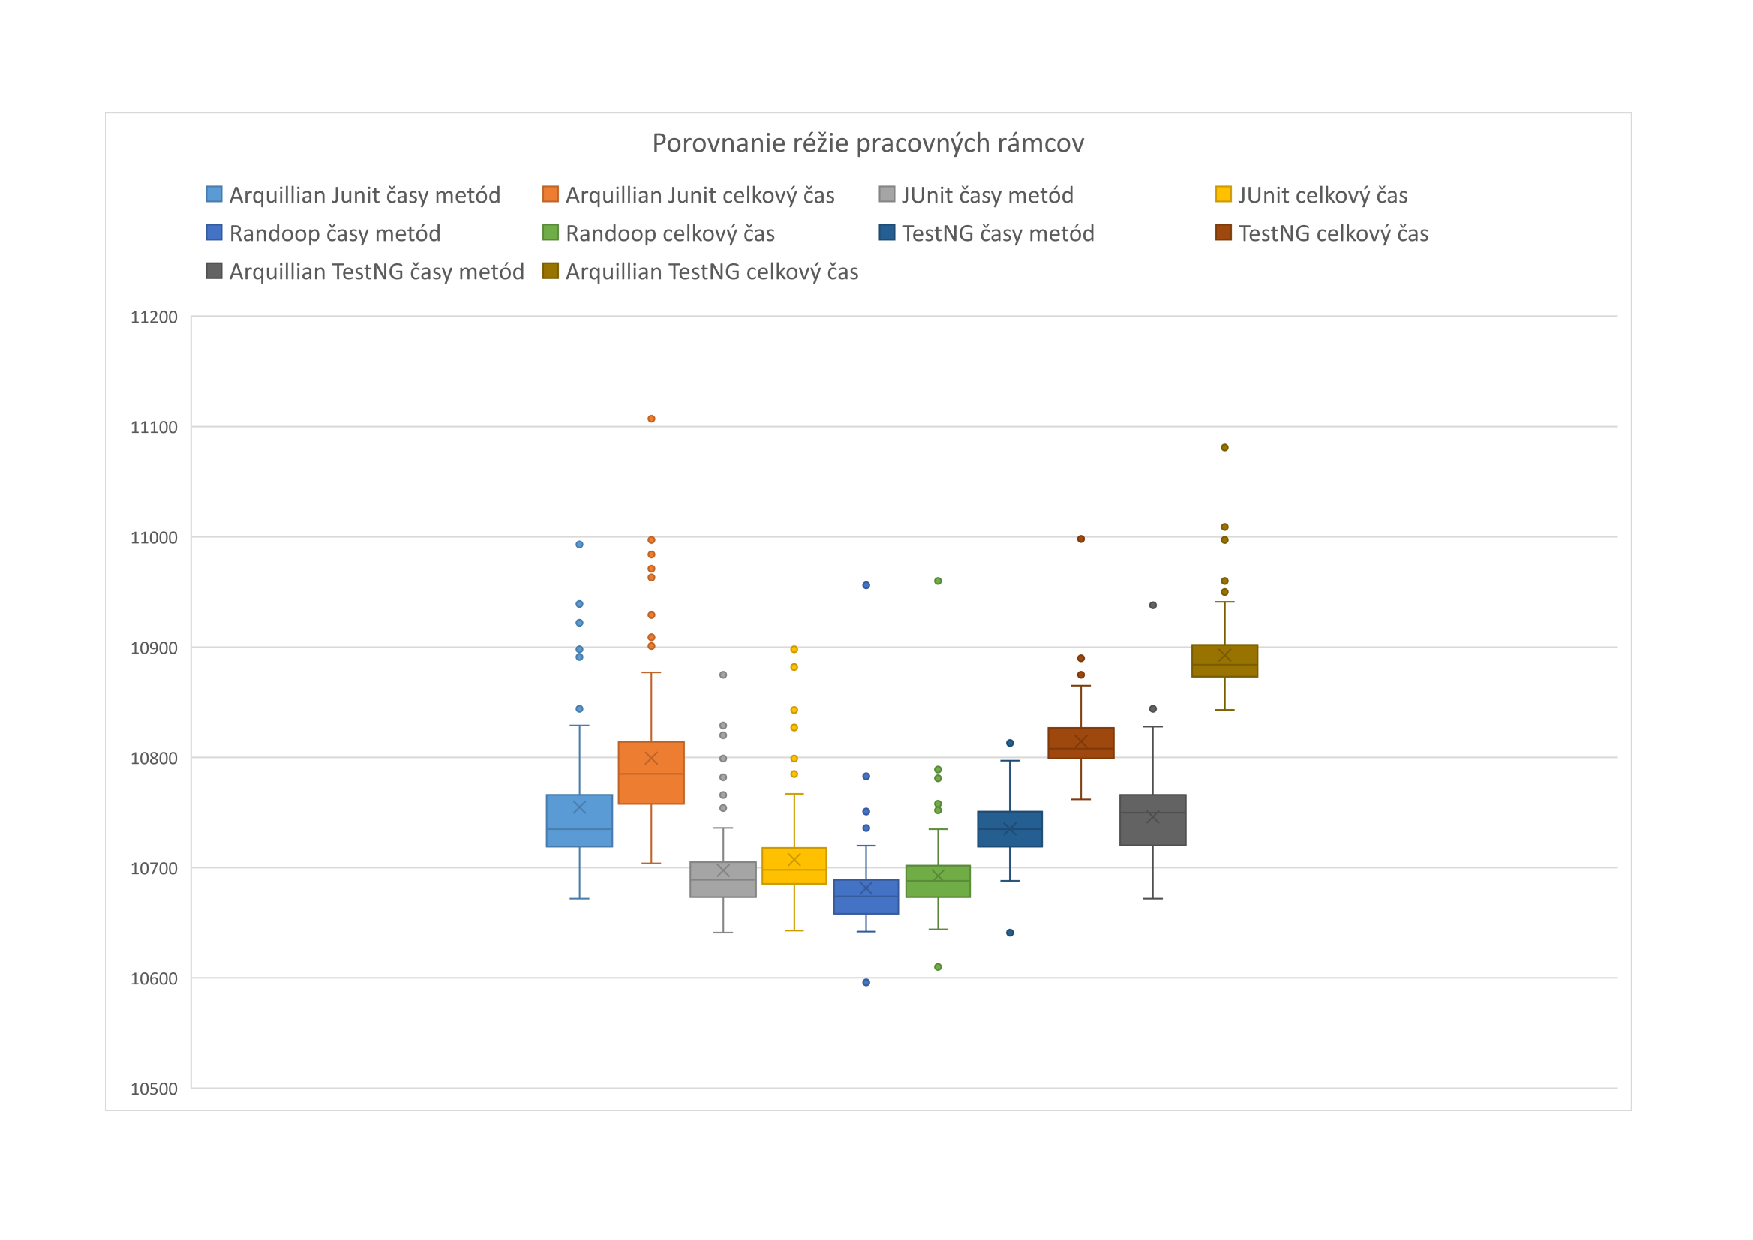
\includegraphics[width = 500pt, trim = 0pt 50pt 0pt 50pt]{graf_rezia}
		\newline
		\tiny Obr. 1. Porovnanie súčtu času metód pri testovaní a celkového času testu aj s inicializáciou.
	\end{center}
	
	Pri sekvenčných testoch je evidentné, že testy sú čo sa týka času veľmi podobné (Obr. 2). Čisté JUnit test bez rozšírenia sú na rovnakej úrovni ako vykonávanie tried mimo testu a dokonca aj o niečo rýchlejšie. To môže byť spôsobené chybou merania, pretože neviem zabezpečiť, aby operačný systém na počítači nevykonával aj iné úlohy na pozadí, ktoré môžu mať vplyv na výkon aj keď sme sa snažili tieto nežiadúce vplyvy čo najviac eliminovať. O niečo horšie, ale bez výrazného rozdielu, je na tom Arquillian spúšťaný oboma pracovnými rámcami a samotný TestNG.
	
	\begin{center}
		\hspace*{-1.8cm} 
		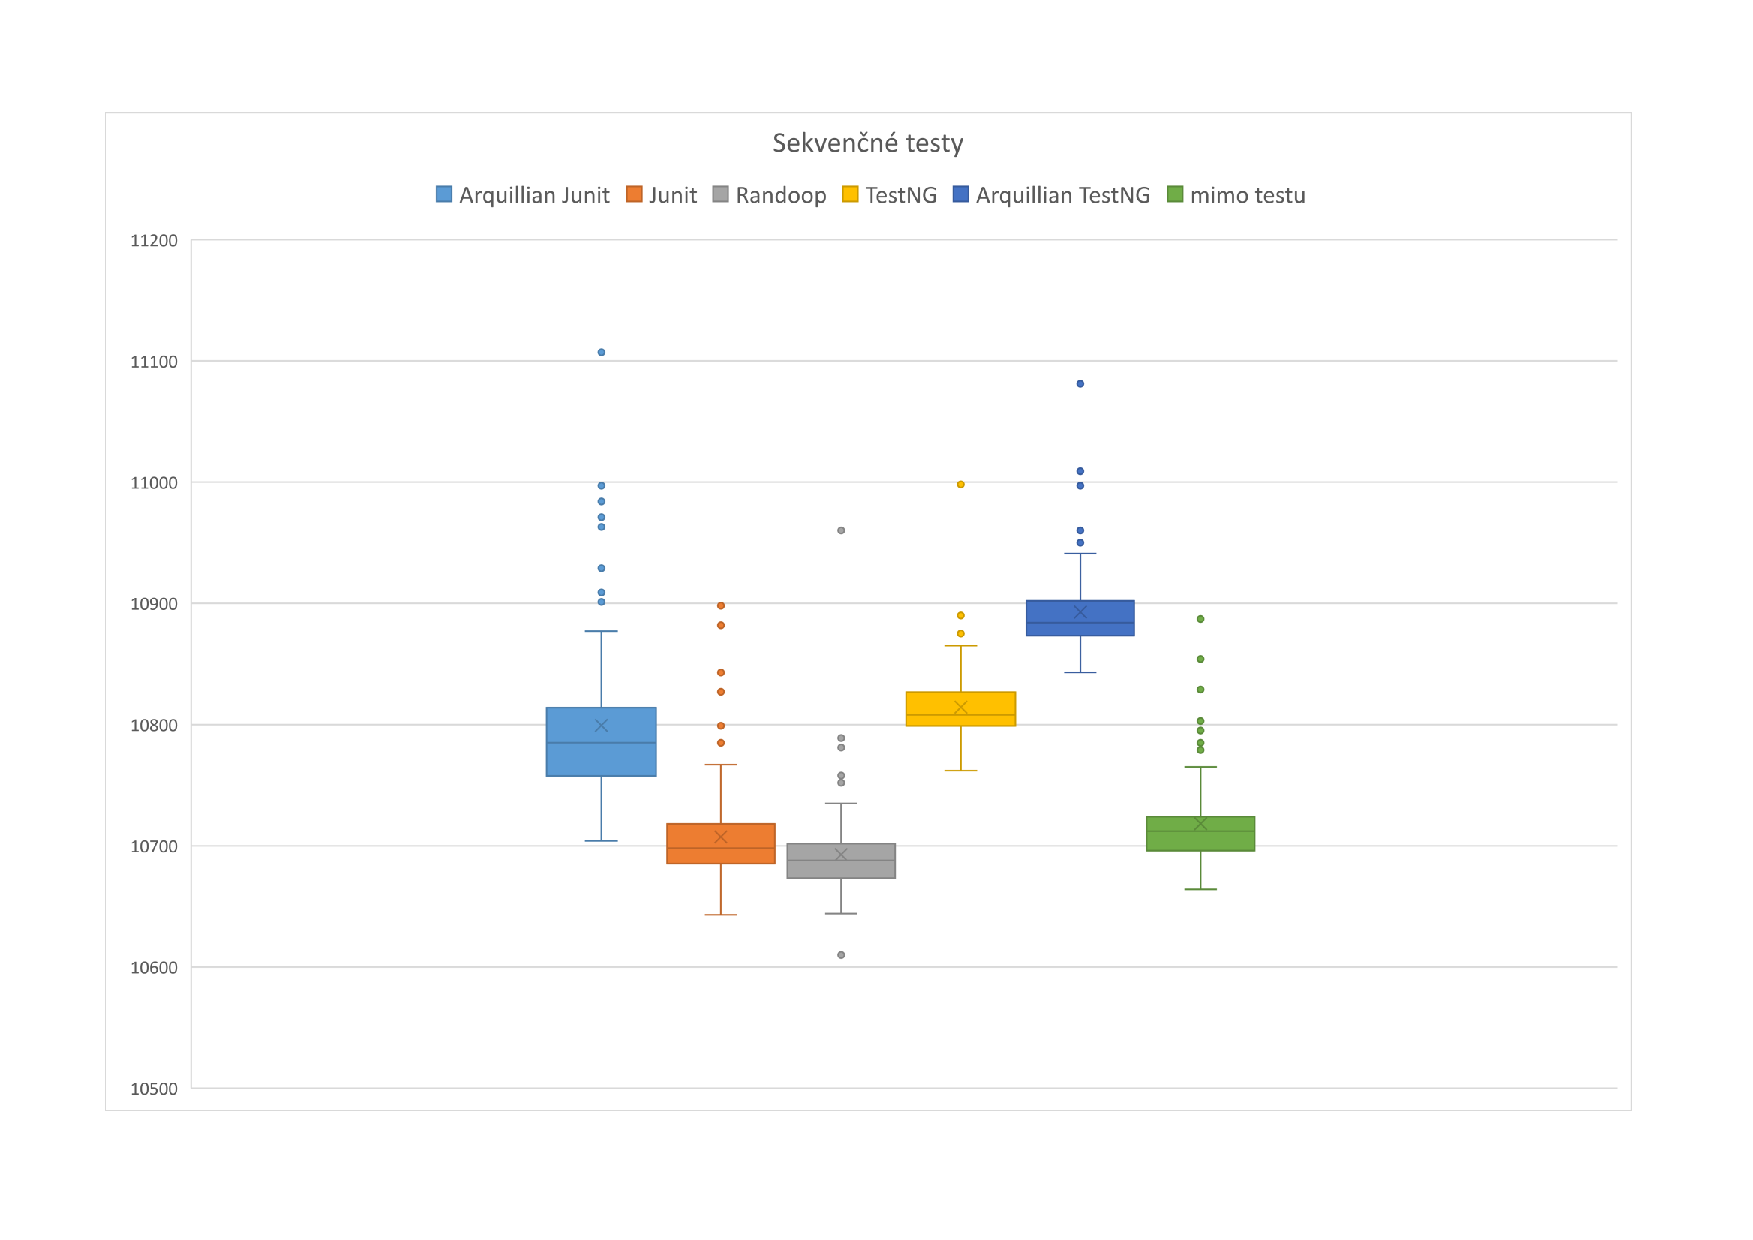
\includegraphics[width = 500pt, trim = 0pt 50pt 0pt 50pt]{graf_sekvencne}
		\newline
		\tiny Obr. 2. Výsledky sekvenčných testov
	\end{center}
	
	Výsledky paralelných testov (Obr. 3) ukazujú presne tie isté výsledky a teda opäť sú na tom najlepšie JUnit pracovné rámce a o niečo horšie Arquillian a TestNG. Pri paralelných testoch je ešte dôležité si všimnúť, že najlepšie časy malo vykonávanie testov v 8 a 16 vláknach (procesor počítača, na ktorom prebiehali testy má 2 jadrá a 4 vlákna). Pri iných počtoch jadier, na ktorých boli testy spúšťané boli časy horšie, čo naznačuje, že je 
	okolo testov dosť réžie, pretože najlepšie využitie bolo až pri 8 vláknach. Keby tam táto réžia nebola a išlo by len o výpočet najlepšie časy by sme dosahovali pri 2, resp. 4 vláknach.
	\begin{center}
		\hspace*{-1.8cm} 
		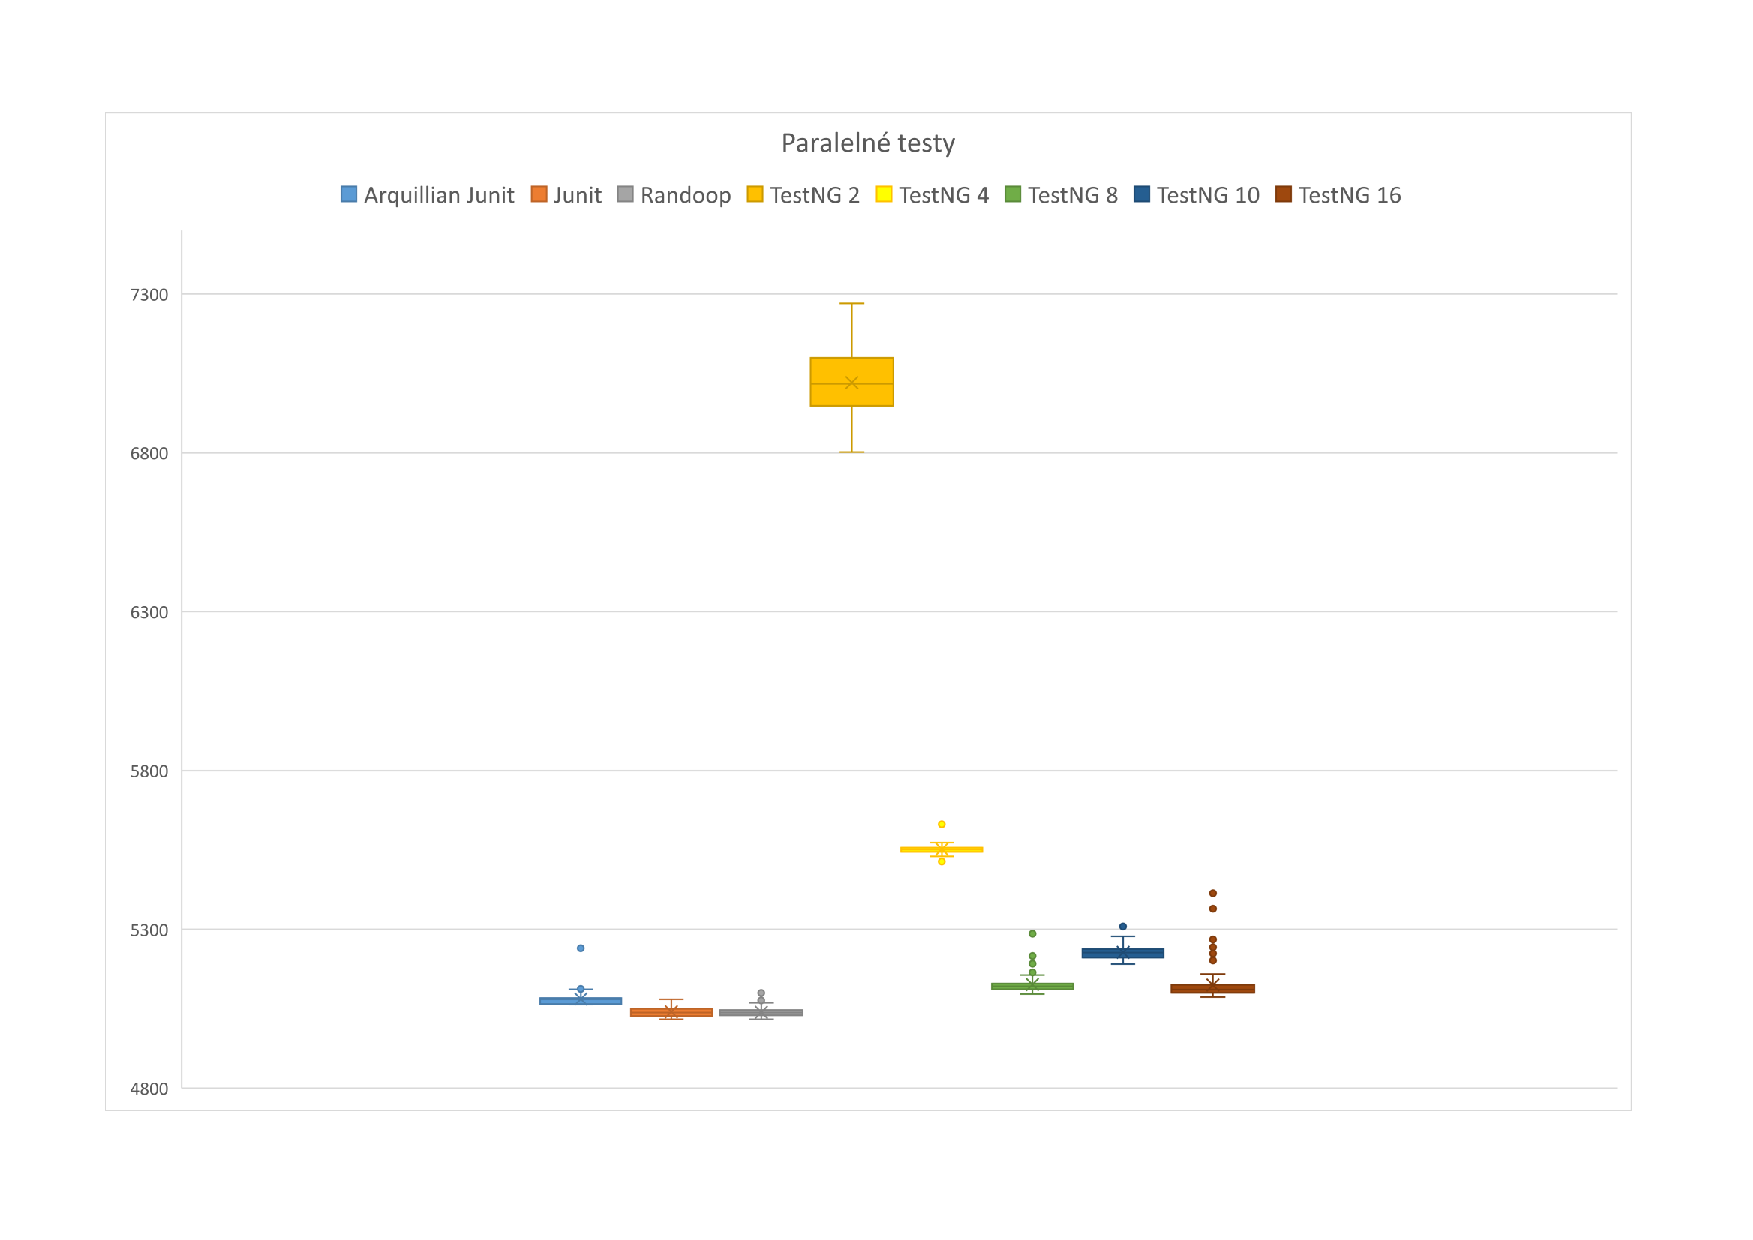
\includegraphics[width = 500pt, trim = 0pt 50pt 0pt 50pt]{graf_paralelne}
		\newline
		\tiny Obr. 3. Výsledky paralelných testov
	\end{center}
	
	Treba ešte dodať k už spomínanej vlastnosti Arquillianu, vytvárať vlastné zostavy, že pri väčších projektoch môže táto vlastnosť urýchliť priebeh testov, pretože v zostave si vieme definovať, ktoré triedu sú pre nás v teste dôležité a ostatné nemusia byť pripojené. Tým pádom by sme vedeli ušetriť čas pri inicializácií testu, najmä ak používame v programe veľa tried s rôznou mierou vzájomnej spolupráce. V našich výsledkoch vplyv tejto vlastnosti nie je vidieť, pretože rozsah nami testovaných tried nebol veľký.
	
	\subsection{Požiadavky na úroveň skúsenosti programátora}
	Využitie základných funkcií testovaných pracovných rámcov si nevyžaduje špecifické skúsenosti programátora, ale pri viacerých funkciách sú určite výhodou skúsenosti, dokonca aj nie priamo súvisiace s programovaním. Najjednoduchším na používanie je JUnit, pretože používa anotácie, ku ktorým sú na internete dostupné návody ako ich používať aj s príkladmi, prípadne triedy na vytvorenie zostáv spúšťaných testov. Teda netreba sa poznať syntax ničoho okrem programovacieho jazyka a potrebné anotácie. O niečo viac skúseností treba na používanie Randoop kvôli absencií grafického prostredia. Vyžaduje si skúsenosti s prácou v príkazovom riadku. Stačí aj základná úroveň, ale v súčasnosti to už nie je nevyhnutnosť ovládať, ak chce človek programovať. TestNG tiež nevyžaduje žiadne skúsenosti okrem programovania pre využitie základných funkcií, ale na plnohodnotné používanie treba vedieť písať konfiguračné xml súbory. Pre programátora by nemali tieto súbory spôsobovať problém, ale treba skúsenosti na to, aby v nich vedel čítať a písať ich. Najnáročnejším na skúsenosti z vybraných pracovných nástrojov je Arquillian, pretože vyžaduje orientáciu v Maven projekte a aj poznanie špecifík JUnit, resp. TestNG podľa toho ako ho chceme používať.
	

	\newpage
 	\thispagestyle{plain}
	\section{Vyhodnotenie výsledkov testovania}
	Vyhodnetie robíme vždy najprv pre JUnit a TestNG, v ktorom budeme hodnotiť ich pre a proti a následne budú ostatné vybrané pracovné rámce porovnané s nimi. Za každú kategóriu hodnotenia je maximálny počet bodov 5. Vzhľadom na zistenú veľkú podobnosť vo všetkých vlastnostiach prispôsobíme tomu aj systém hodnotenia. Hodnotenie by prebiehalo tak, že základné pracovné rámce by dostávali z každej kategórie 2 a 4 body (lepší z nich 4 a horší 2). A ostatné pracovné rámce by následne dostávali 1 bod ak by boli horšie ako horší zo základných, 3 body ak by boli niekde medzi nimi, 5 bodov ak by boli lepšie ako lepší zo základných a rovnaký počet ako niektorý zo základných ak v danej vlastnosti nebude pozorovateľný rozdiel.
	
	Jediná objektívne merateľná vlastnosť v našom testovaní je čas testovania všetkých testovacích metód v testovacích triedach. Podľa výsledkov môžeme jednoznačne za čas prideliť 4 body JUnitu, pretože jednoznačne dosahoval lepšie časy ako TestNG ako to možno vidieť aj v grafoch v predchádzajúcej kapitole. Randoop dostáva 4 body rovnako ako JUnit, lebo aj pri sekvenčných aj pri paralelných mali veľmi podobné výsledné časy. Arquillian je ťažšie zaradiť na správne miesto, keďže je zároveň medzi JUnit a TestNG aj horší ako TestNG (podľa toho pod akým pracovným rámcom sa spúšťa) a v paralelných testoch bol testovaný len ako JUnit. Vzhľadom na fakt, že pri väčších projektoch dokáže šetriť čas pomocou zostáv sme sa rozhodli udeliť mu 3 body.
	
	Ostatné vlastnosti sa už nedajú hodnotiť do takej miery objektívne ako čas, ale máme snahu hodnotiť ich podľa toho, čo sa v praxi medzi programátormi javí ako lepšia voľba.
	
	V prehľadnosti dostáva 4 body TestNG preto, že poskytuje možnosť anotácií v kóde, ale aj použitie konfiguračného xml súboru, ktoré sú v súčasnosti považované za štandard v oblasti konfigurácie v informatike a sú aj prehľadné. JUnit teda dostáva 2 body a rovnako aj Randoop, pretože konfigurácia je možná len cez anotácie. Arquillian sa opäť dostáva medzi tieto pracovné rámce, pretože kombinuje v sebe vlastnosti oboch pracovných rámcov, ale nedokáže využiť výhody oboch súčasne.
	
	V univerzálnosti je jednoznačne lepším pracovným rámcom TestNG, pretože dokáže spúšťať rovnako svoje triedy testov, ale bez nevyhnutnosti zmeny aj JUnit testy. Naopak JUnit vie spúšťať len svoje testy a preto dostáva 2 body. Arquillian dostáva 4 body rovnako ako TestNG pretože sa dokáže byť spustený aj ako JUnit test aj ako TestNG test. Ostal nám Randoop, ktorý generuje len JUnit testy a preto dostáva 2 body rovnako ako JUnit.
	
	Pri správe spúšťania testov v možnostiach v podstate nie sú rozdiely. Všetky pracovné rámce umožňujú vytvoriť vlastné triedy a aj skupiny testov, ktoré môžu byť spúšťané tak ako chceme. Rozdiel je len v tom ako sa tieto triedy a skupiny špecifikujú, ale to patrí do hodnotenia inej kategórie. Vzhľadom na takúto situáciu sme v tejto kategórií urobili výnimku a všetky pracovné rámce dostanú zhodne po 5 bodov.
	
	Bez zásahu do zobrazovania výsledkov a odhliadnutia od zobrazenia výsledkov prostredníctvom zásuvného modulu je jediný rozdiel medzi pracovnými rámcami v tom, že TestNG vypisuje výsledky na konzolu. Výpis na konzolu môže byť žiaduci aj nie takže sa nedá jednoznačne určiť čo je lepšie. Výraznejší rozdiel môžeme vidieť pri listeneroch. TestNG listener poskytuje viac metód a pomocou používaného rozhrania aj podrobnejšie informácie. Aby sme teda ostali pri dohodnutom hodnotení tak všetky pracovné rámce používajúce TestNG dostanú 4 body a JUnit 2 body.
	
	Body za potrebné programátorské skúsenosti pridelíme podľa toho ako sme zoradili pracovné rámce v predchádzajúcej kapitole. Najjednoduchší je JUnit a získava teda podľa nášho bodovania 4 body. Po ňom nasleduje Randoop s 3 bodmi, TestNG s 2 a nakoniec Arquillian s 1 bodom.	
	
	Pretože jediný pracovný rámec, ktorý vie generovať testy automaticky je Randoop dostáva za túto kategóriu 5 bodov. Ostatné pracovné rámce dostávajú 0, pretože je to veľmi užitočná vlastnosť, ale oni ňou nedisponujú.

	\begin{center}
		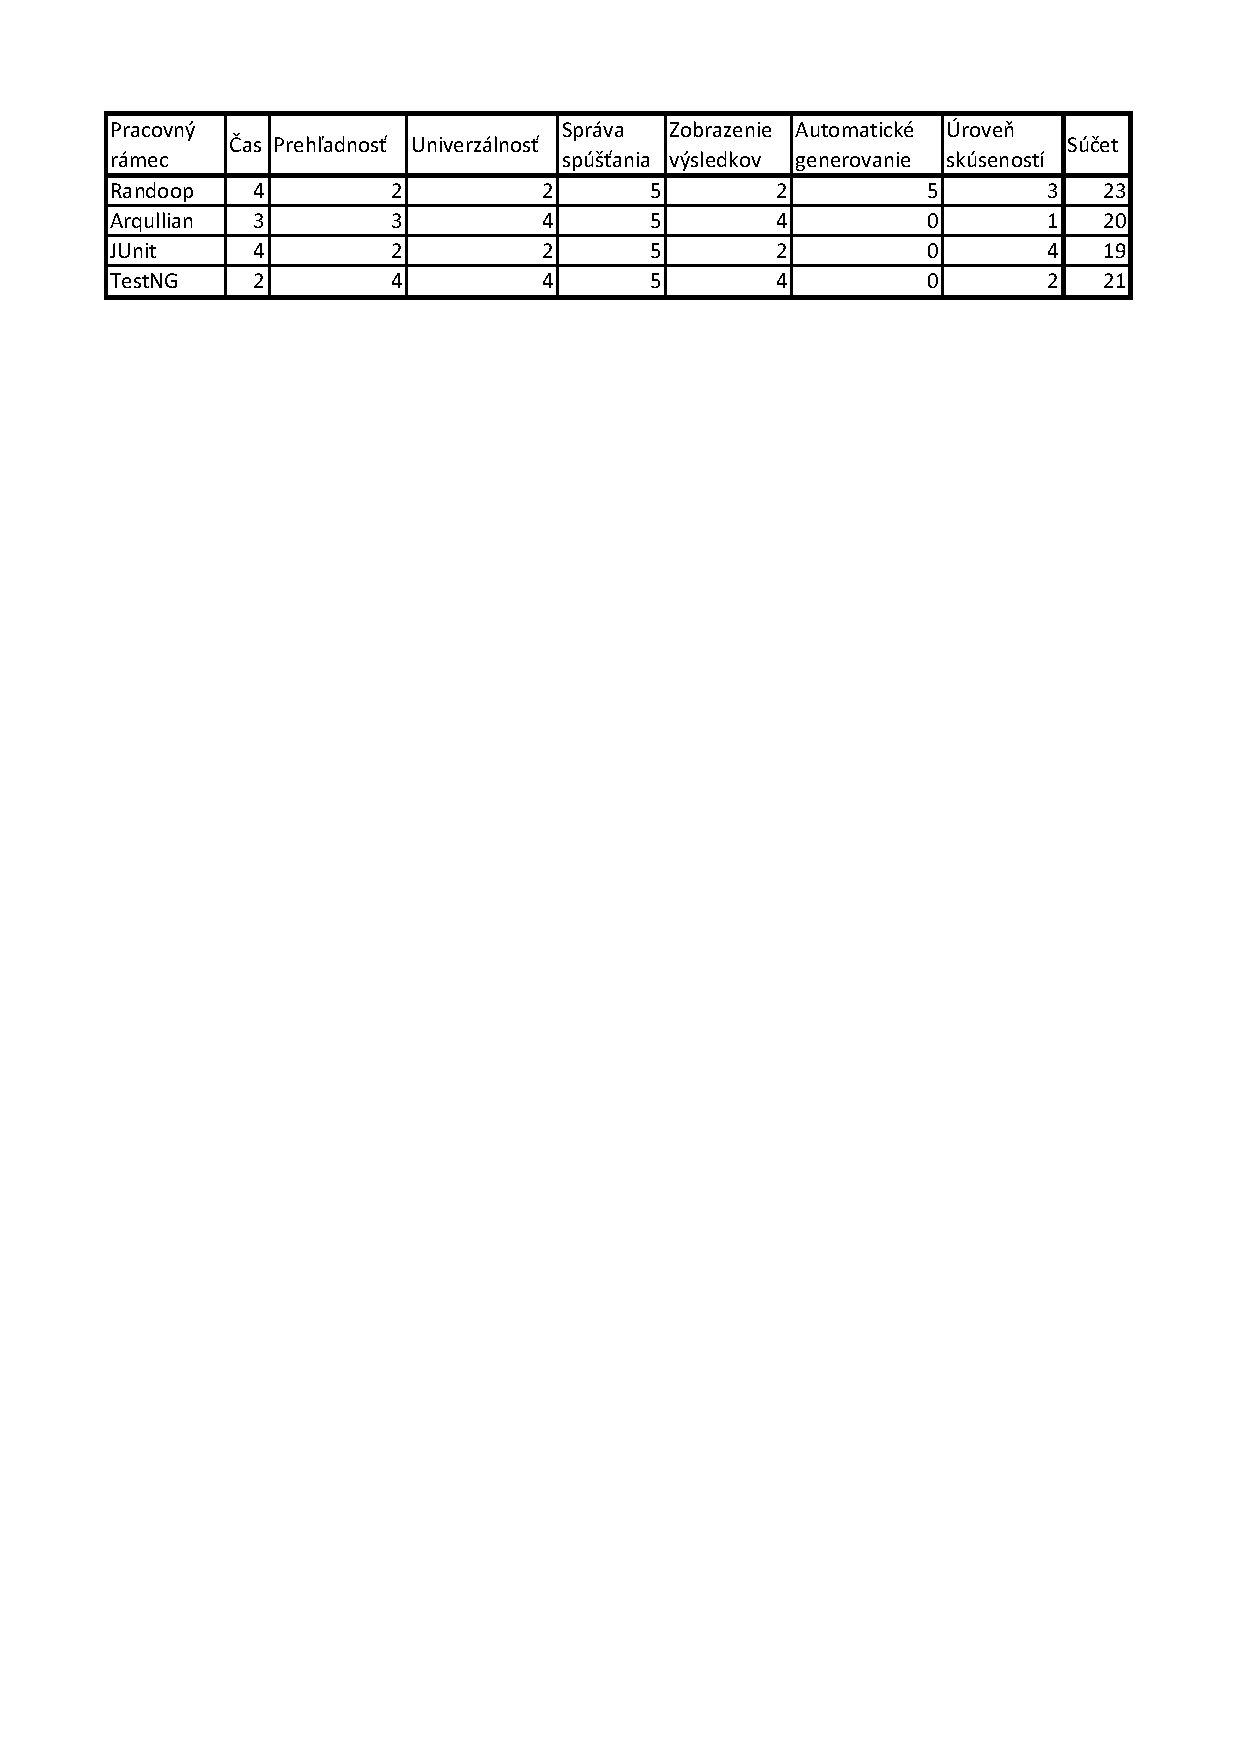
\includegraphics[width = 400pt, trim = 0pt 700pt 0pt 0pt]{tabulka}
		\newline
		\tiny Tab. 1. Výsledok hodnotenia
	\end{center}
		
	\subsection{Vhodnosť použitia pracovných rámcov podľa charakteristiky projektu}
	Vyhodnotením sme získali porovnanie pracovných rámcov podľa rôznych kritérií, ale každý projekt má iné potreby a preto treba doplniť, že ten ktorý z nášho testu vyplýva ako najlepší, nemusí byť najlepšia voľba vždy. Randoop vďaka tomu, že vie generovať testy je podľa hodnotenia najlepší, ale pri projektoch veľkého rozsahu by vygeneroval obrovské množstvo testov, z ktorých väčšina by bola zbytočná lebo by sa v nich opakovane testovalo viackrát to isté. Vo veľkých projektoch by bolo potom treba kontrolovať a vylúčiť zbytočné testy a od istej hranice je vhodnejšie napísať si ich ručne.
	
	Druhým v našom poradí je TestNG, ktorý umožňuje písať testy a zároveň má veľmi dobre rozpracovanú možnosť konfigurácie testov rôznymi spôsobmi. Je vhodný pre malé, ale aj väčšie projekty. Pri väčších projektoch si vyžaduje viac skúseností programátora, pretože vytvoriť správnu konfiguráciu pre veľký projekt nie je jednoduché.
	
	Arquillian je výborným nástrojom pre veľké projekty, pretože dokáže rozdeliť testovanie na menšie časti a tým ušetriť čas. Jeho nevýhodou pri malých projektoch je závislosť na veľa knižniciach čo čiastočne komplikuje jeho používanie, aj keď vďaka integrácií v Maven projekte to nie je náročné. Vo veľkých projektoch by sa aj réžia, ktorú má mala odstrániť a mal by mať oproti ostatným nástrojom v tomto smere výhodu, ale to už nebolo súčasťou nášho testovanie a preto to ostáva len v rovine predpokladu.
	
	JUnit vyšiel z nášho hodnotenia najhoršie, ale je to dobrý nástroj pre začiatočníkov v jednotkovom testovaní. Je jednoduchší na používanie, pretože nepoužíva žiadne externé súbory a všetko sa dá nastaviť a prispôsobiť z vývojového prostredia. Čo sa týka rozsahu projektu je na tom rovnako ako TestNG.
	
	\newpage
 	\thispagestyle{plain}
	\section{Záver}
	V práci sme analyzovali testovanie softvéru a zamerali sme sa na analyzovanie jednotkového testovania. Analýzou vlastností jednotkového testovania sa nám podarilo vytvoriť teoretický koncept ideálneho pracovného rámca pre jednotkové testovanie. Snažili sme sa vlastnosti určovať tak, aby sme hovorili o uskutočniteľných vlastnostiach, resp. už skutočných vlastnostiach, ale zatiaľ nie spojených do jedného pracovného rámca, a nebolo to niečo nemožné v realite. Tieto vlastnosti sme porovnali s dostupnými informáciami o vlastnostiach niekoľkých existujúcich pracovných rámcov zo skupiny xUnit. Vybrali sme viacero pracovných rámcov pre jazyk Java. Vlastnosti týchto pracovných rámcov sme porovnali s vlastnosťami ideálneho pracovného rámca. Zhodnotili sme, ktoré vlastnosti pracovné rámce implementujú a ktoré naopak ešte nie alebo ich implementujú len čiastočne. Na základe predbežného hodnotenia, nepotvrdeného testami sa javil najlepší pracovný rámec Randoop. Po testoch na vybraných pracovných rámcoch sa tento predpoklad potvrdil a podarilo sa nám zoradiť vybrané pracovné rámce podľa vhodnosti použitia a zároveň určiť, na ktoré typy projektov sú jednotlivé pracovné rámce vhodné.
	
	Pracovné rámce sa majú stále ešte v čom zlepšovať. Veľmi nápomocným zlepšením by v praxi bola určite možnosť automatického spúšťania len tých testov, ku ktorým sa viaže nejaká zmena v zdrojovom kóde od posledného testovania. Taktiež by bolo posunom vpred aj rozšírenie možnosti automatického generovania testov, pretože teraz je to viazané v podstate len na jeden pracovný rámec, aj keď sa dajú tieto testy za istých podmienok spustiť aj pomocou iných pracovných rámcov, ale vieme tým pádom využiť pri generovaní len výhody jedného z nich. 

%	\section{Ciele a záver práce}
	
%	V práci sme analyzovali testovanie softvéru a zamerali sme sa na analyzovanie jednotkového testovania. Analýzou vlastností jednotkového testovania sa nám podarilo vytvoriť teoretický koncept ideálneho pracovného rámca pre jednotkové testovanie. Snažili sme sa vlastnosti určovať tak, aby sme hovorili o uskutočniteľných vlastnostiach, resp. už skutočných vlastnostiach, ale zatiaľ nie spojených do jedného pracovného rámca, a nebolo to niečo nemožné v realite. Tieto vlastnosti sme porovnali s dostupnými informáciami o vlastnostiach niekoľkých existujúcich pracovných rámcov zo skupiny xUnit. Vybrali sme viacero pracovných rámcov pre jazyk C\# a aj viacero pre jazyk Java. Vlastnosti týchto pracovných rámcov sme porovnali s vlastnosťami ideálne pracovného rámca. Zhodnotili sme, ktoré vlastnosti pracovné rámce implementujú a ktoré naopak ešte nie alebo ich implementujú len čiastočne. Na základe zhodnotenia sme potom vedeli určiť, ktorý pracovný rámec má najviac spoločných vlastností s ideálnym a teda má k nemu najbližšie. Aj pre jazyk C\# aj pre jazyk Java bol najlepší pracovný rámec Randoop, resp. Randoop.NET.
	
%	Cieľom našej práce je vytvoriť projekt v takom rozsahu, aby sme mohli otestovať a zhodnotiť tento pracovný rámec aj v skutočnosti. Našim cieľom je vyskúšať vlastnosti tie vlastnosti pracovného rámca, o ktorých sa v práci diskutuje. Na jednom projekte sa nám pravdepodobne nepodarí do hĺbky otestovať všetky jeho vlastnosti, ale chceme otestovať každú aspoň čiastočne a tie pri ktorých to bude možné aj do hĺbky. Vzhľadom na to, že projekt ešte nemáme špecifikovaný nevieme konkretizovať ktoré vlastnosti a ako bude možné otestovať. Testovať budem pracovné rámce Randoop a Randoop.NET a projekt bude implementovaný v oboch jazykoch (C\#, Java).
	
%	\newpage
%	\section{Časový plán do odovzdania práce v letnom semestri}
%	\begin{itemize}
%		\item \textbf{december 2015} - špecifikácia projektu, na ktorom budem implementovať testovanie
%		\item \textbf{január a február 2016} - implementácia projektu, implementácia testov vo vybraných pracovných rámcoch
%		\item \textbf{marec 2016} - testovanie projektu pracovnými rámcami a zhromažďovanie výsledkov testov pre účely zhodnotenia
%		\item \textbf{apríl 2016} - zhodnotenie a porovnávanie pracovných rámcov
%		\item \textbf{máj 2016} - dokončovanie práce a odovzdanie do 10.5.2016
%	\end{itemize}
    \newpage
 	\pagestyle{fancy}
 	\fancyhf{}
 	\fancyfoot[CE,CO]{\thepage}
 	\bibliography{literatura}
 	\bibliographystyle{plain}
 	
 	\newpage
 	\thispagestyle{plain}
 	\part*{Prílohy}
	\renewcommand\thesection{\Alph{section}}
	\setcounter{section}{0}
 	\section{Technická dokumentácia}
 	
 	Priebeh testovania zobrazujú diagramy na obrázkoch 6 a 7. Na obrázku 6 je diagram vykonávania testu pre každú testovaciu triedu. Ako môžeme vidieť každá trieda sa vykonáva 100-krát, meriame čas pred spustením a po spustení testu a pred spustením sa priradí k spúšťaču správny listener (Obrázok 5).
 	
 	%\begin{center}
 	%	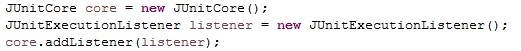
\includegraphics[width = 200pt]{junit}
 	%	\newline
 	%	\tiny Obr. 4. Naviazanie JUnit listenera.
 	%\end{center}
 	
 	\begin{center}
 		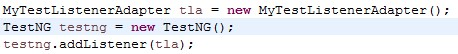
\includegraphics[width = 320pt]{testng}
 		\newline
 		\tiny Obr. 5. Naviazanie TestNG listenera.
 	\end{center}
 	
 	V programe je tento diagram implementovaný pomocou 4 tried. 2 triedy pre TestNG a 2 pre JUnit a z týchto dvojíc je vždy jedna na sekvenčné a jedna na paralelné testy. Rozdelené sú pre to, že sú tam odlišnosti v zdrojovom kóde v spúšťaní medzi týmito pracovnými rámcami a aj medzi paralelným a sekvenčným spustením testov, ale postup vykonávanie je veľmi podobný. Aby nevznikla zbytočná duplicita tak sme dali celý postup do jedného diagramu. Pri paralelných JUnit testoch sa nenastavuje počet vlákien explicitne, pretože to spúšťač neumožňuje.
 	
 	\begin{center}
 		\hspace*{-2.5cm} 
 		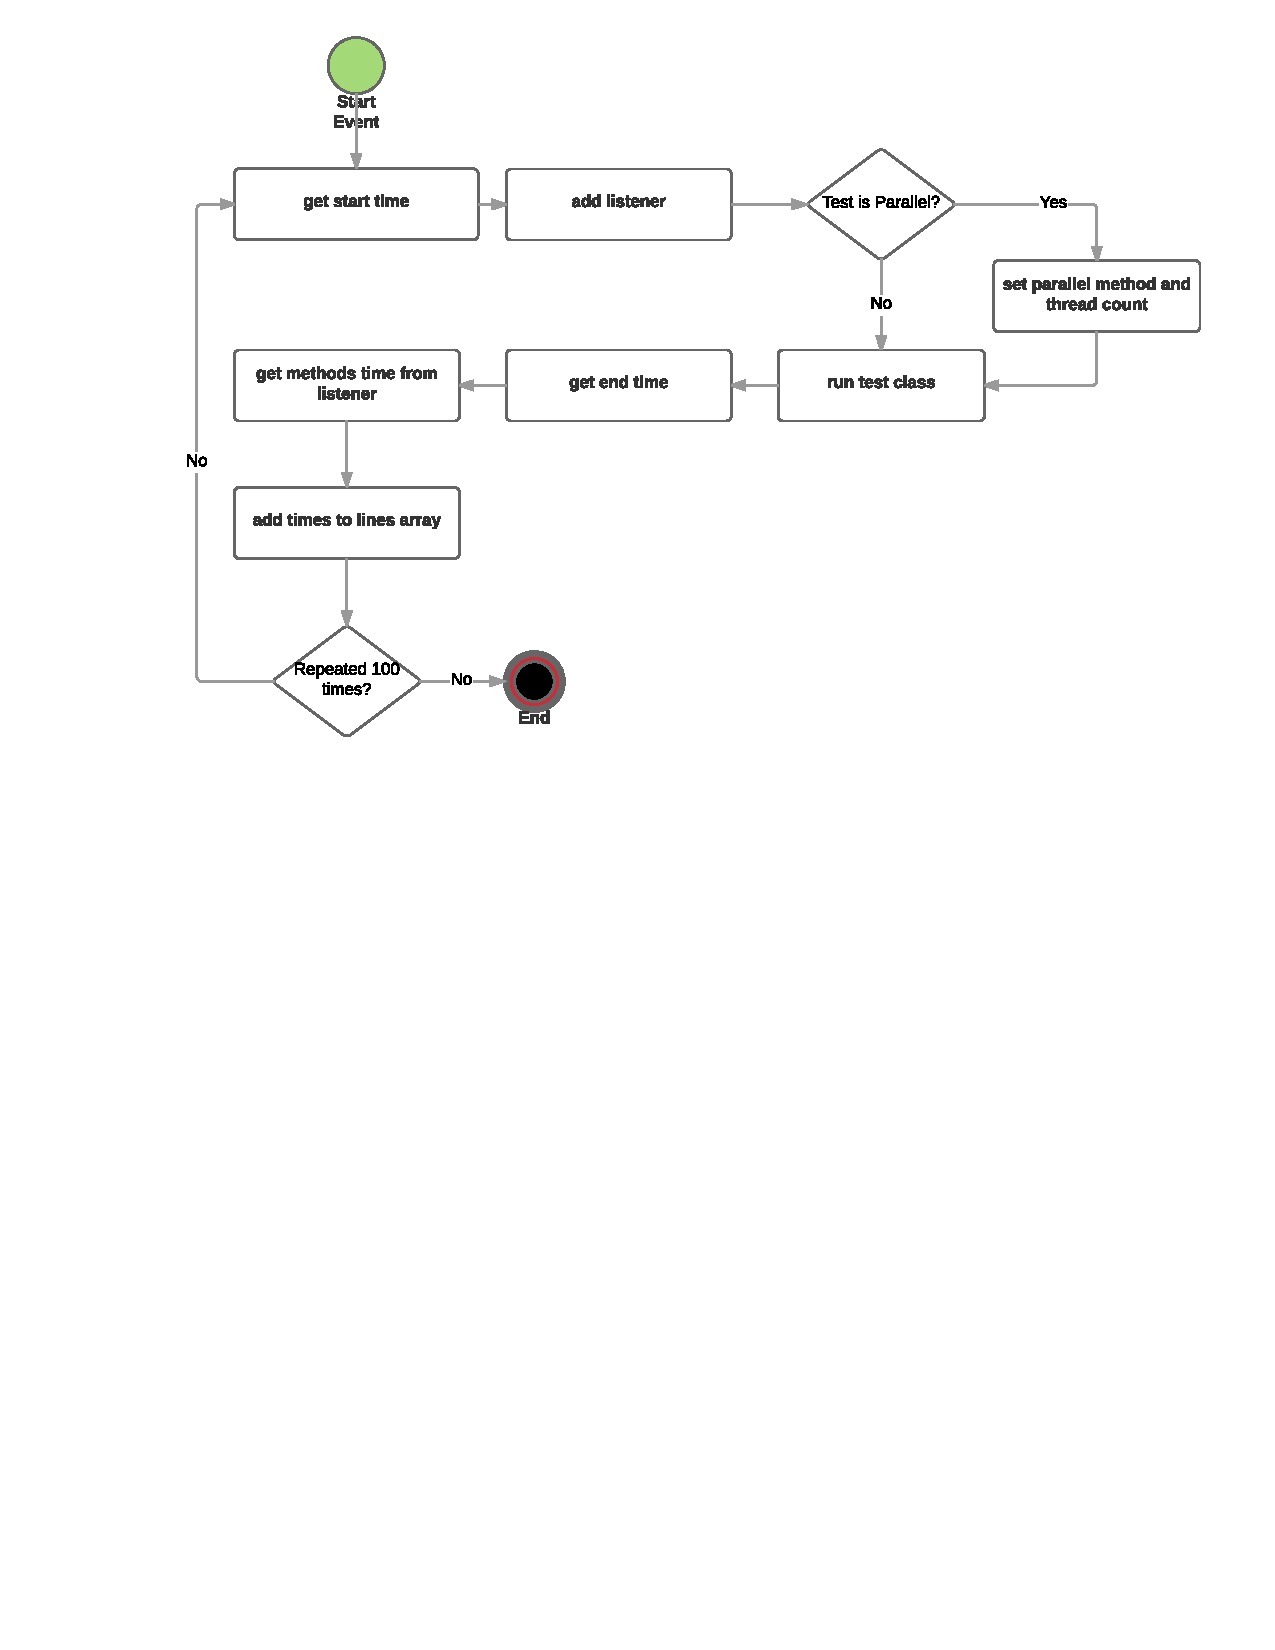
\includegraphics[width = 500pt, trim = 0pt 440pt 0pt 70pt]{test}
 		\newline
 		\tiny Obr. 6. Diagram vykonávania testov.
 	\end{center}
 	
 	Na obrázku 7 je diagram, zobrazujúci priebeh testovania každej triedy. Pred a po každej metóde sa zisťuje čas, aby sme vedeli zistiť ako dlho trvá jej vykonávanie. To isté sa vykoná aj pred vykonaním prvej a poslednej metódy v celej triede pre získanie celkového času.
 	
 	\begin{center}
 		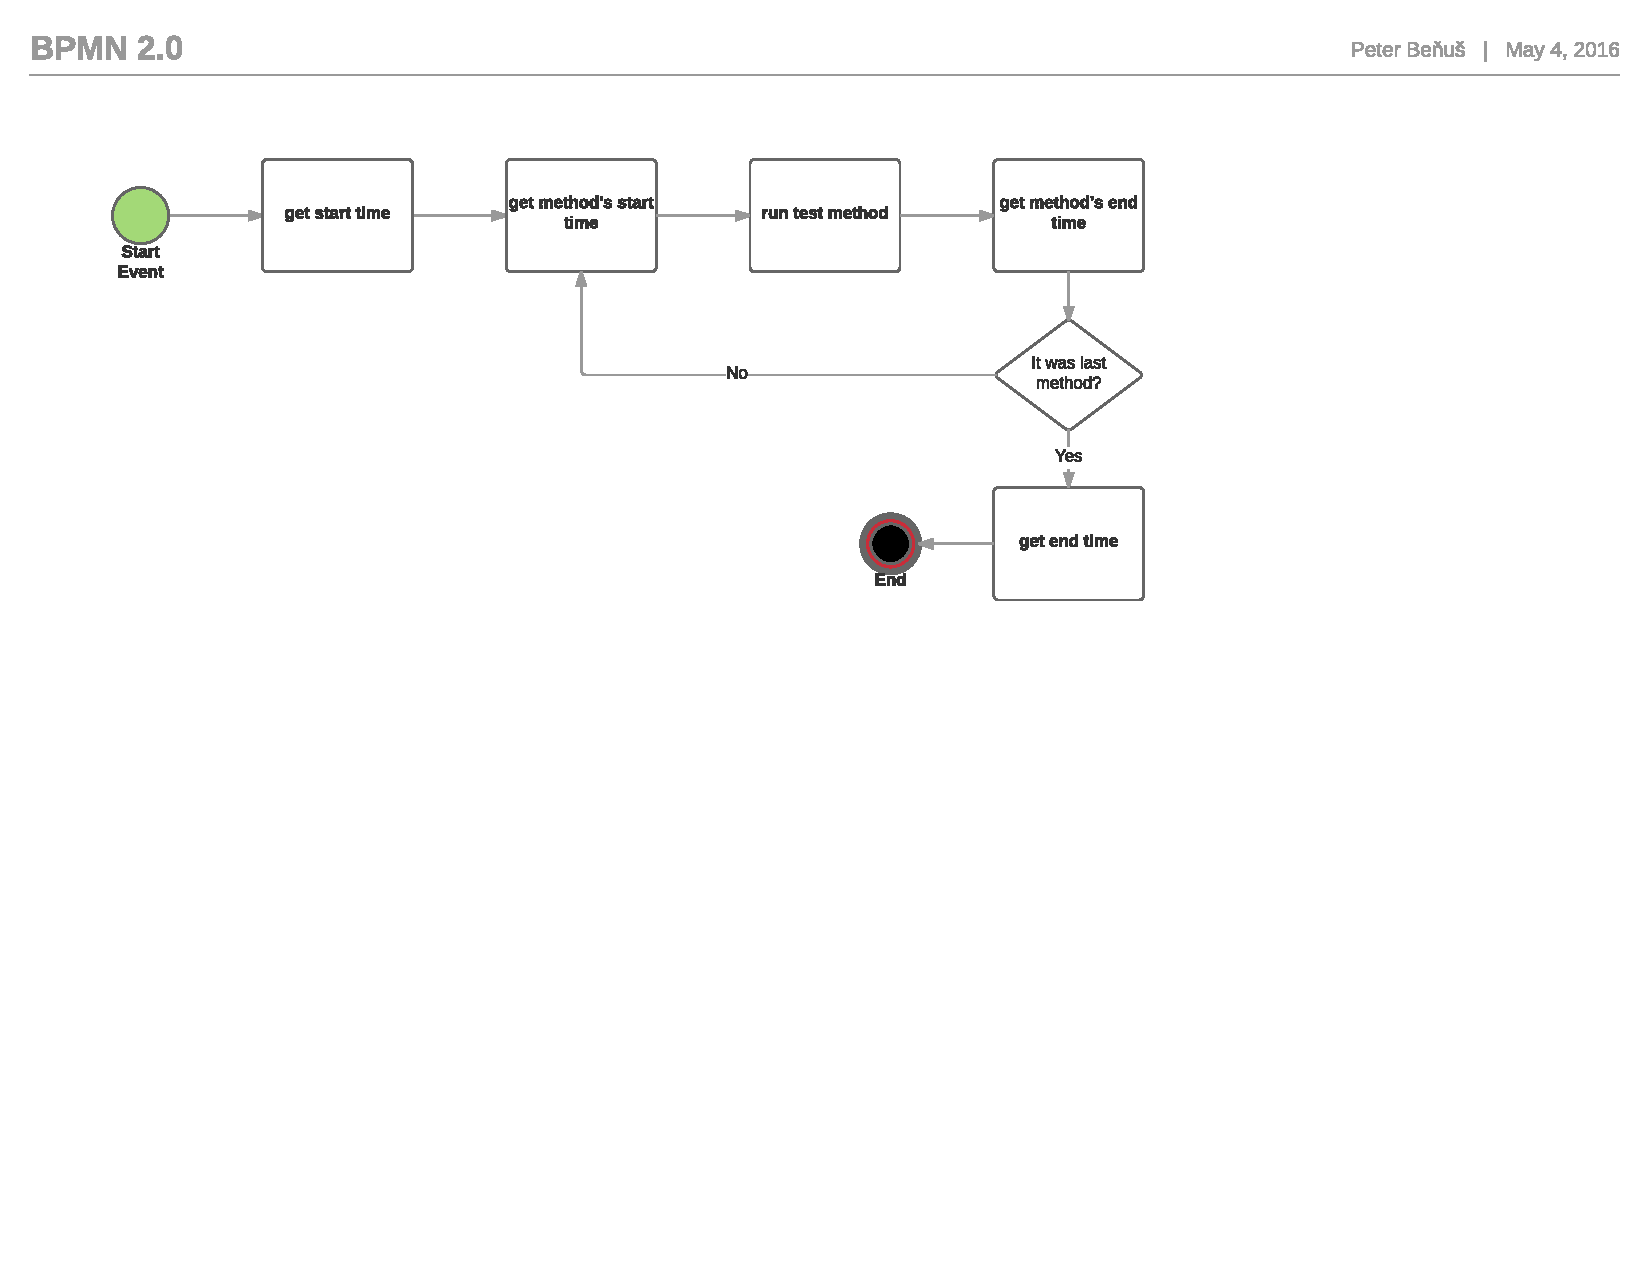
\includegraphics[width = 500pt, trim = 0pt 315pt 0pt 40pt, clip]{listener}
 		\newline
 		\tiny Obr. 7. Diagram priebehu testu testovacej triedy.
 	\end{center}
 	
 	Rovnakým spôsobom boli merané aj časy vykonávania testov mimo testovania, ale boli použité samostatné triedy.
 	
 	Na obrázku 8 je príklad jednej z testovacích metód pracovného rámca TestNG, použitých na testovanie prototypu. Testovacie metódy vždy vytvoria objekt jednej z tried, ktoré testujeme a následne volajú metódy tejto triedy. Metódy sú volané v rámci jednej testovacej metódy niekedy aj opakovane, buď s rôznymi alebo s rovnakými argumentami. Testuje sa tým, či vracia program vždy správne hodnoty aj po viacnásobnom opakovaní volania tej istej metódy.
 	
 	\begin{center}
 		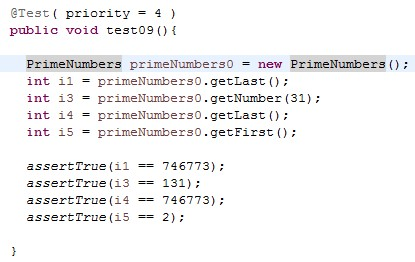
\includegraphics[width = 350pt]{priklad_testu}
 		\newline
 		\tiny Obr. 8. Diagram priebehu testu testovacej triedy.
 	\end{center}
 	
 	Okrem testovacích tried a listenerov, ktorých modely sú na diagramoch obsahuje projekt aj dve testované triedy. Tieto triedy počítajú prvočísla a ich metódy sú volané v testovacích metódach už spomínaných tried.
 	
 	%Na začiatku práce sme zúžili okruh, na ktorý sa v rámci témy budeme zameriavať na jednotkové testovanie. Tým začínala analytická časť práce, v ktorej sme hľadali dostupné pracovné rámce pre jazyky C\# a Java. Po analytickej časti sme sa rozhodli zamerať na jazyk Java a implementovali sme jednotkové testy pre viacero pracovných rámcov. Testy boli implementované pomocou generatívneho pracovného rámca Randoop a vývojového prostredia Eclipse Mars.2. Používali sme Java virtuálny stroj verzie 7, update 80. Testy boli po implementácií opakovane spúšťané v cykle volaním zo zdrojového kódu programu. Zaznamenávali sme čas, ktorý testy potrebovali na vykonanie a následne sme získané dáta vyhodnotili. Okrem vyhodnocovania času sme vyhodnocovali aj iné vlastnosti pracovných rámcov, ktoré priamo ovplyvňujú prácu s nimi. Na základe tohto hodnotenia sme zostavili rebríček pracovných rámcov podľa ich vlastností. Prílohou k práci sú aj zdrojové kódy testov a testovaných tried a aj výsledky v xlsx súbore s presnými časmi testov. Aby sme zabezpečili čo najmenšie odchýlky počas testovania, počas testov neboli na počítači spustené žiadne aplikácie okrem Eclipse, bol napojený na zdroj elektrickej energie, odpojený od internetu(aby sme zabránili operačnému systému alebo aplikácií bežiacej na pozadí sťahovať a inštalovať aktualizácia a pod.) a v možnostiach napájania bol nastavený maximálny výkon.
 	
 	\newpage
 	\sloppy
 	\section{Používateľská príručka}
 	
 	Návod na spustenie experimentu, ktorého zdrojový kód je na priloženom médiu.
 	
 	\begin{enumerate}
 		\item Stiahnuť a nainštalovať virtuálny Java stroj. My sme používali verziu 7, update 80, ale možnosť spustenia by nemala ovplyvniť ani iná, kompatibilná verzia. Je možné ju stiahnuť tu: \url{http://www.oracle.com/technetwork/java/javase/downloads/jre7-downloads-1880261.html}.
 		\item Stiahnuť a nainštalovať vývojové prostredie Eclipse Mars.2 z \url{https://eclipse.org/downloads/}.
 		\item Stiahnuť a nainštalovať Apache Maven z  \url{https://maven.apache.org/download.cgi}.
 		\item Stiahnuť Randoop-2.1.4.jar z \url{https://github.com/randoop/randoop/releases/tag/v2.1.4}.
 		%\item Vygenerovať testy pomocou Randoop. Použili sme tento príkaz v príkazovom riadku "java -ea -classpath randoop-2.1.4.jar;target\textbackslash classes\ randoop.main.Main gentests --classlist=classes.txt --outputlimit=100". Príkaz v takomto tvare by mal byť spúšťaný v rovnakej zložke ako projekt alebo treba použiť úplné cesty k súborom namiesto relatívnych. Súbor classes.txt, ktorý používame obsahuje názvy tried, pre ktoré sa majú generovať testy. Podrobnejší návod na použitie Randoop je možné nájsť na \url{https://randoop.github.io/randoop/manual/index.html}.
		%\item Takto vygenerovaná trieda je základom všetkých ostatných testovacích tried.
		\item Testovanie spúšťame spustením triedy RunTests2. Nastavením premennej count na počet opakovaní všetkých testovacích tried.
		\item Namerané časy sa uložia do súboru testy.csv. Pred začiatkom údajov každej spúšťanej testovacej triedy je jej názov a za ním nasledujú názvy metód s časmi metód a celkový čas každého behu.
 	\end{enumerate}
 	
 	
 	%V zdrojových kódov v balíčku benus.peter.bakalarka a v zložke src/main/java sa nachádzajú zdrojové súbory testovaných tried (PrimeNumbers, PrimesPrint). Okrem nich sú tam ďalšie dva súbory, slúžiace na meranie času vykonávania tých istých operácií ako pri testovaní, ale bez kontroly toho či sú výstupy správne. Trieda Methods obsahuje metódy korešpondujúce s testovacími a metódu, ktorá zavolá všetky tieto metódy a zároveň zistí čas potrebný na ich vykonanie. 
 	
% 	V tom istom balíčku v zložke src/test/java sa nachádzajú zdrojové súbory testovacích tried, listenery, súbor test.xml a triedy na opakované spúšťanie, ktorými sme získavali údaje pre vyhodnotenie. Názvy tried sú vždy odvodené od názvu pracovného rámca, okrem Randoopu, ktorý triedy generuje. Trieda z názvom RegressionTest je vlastne skupina testov vygenerovaných Randoopom, aby bolo možné ich naraz spúšťať. Trieda RegressionTest0 obsahuje vygenerované testovacie metódy pracovným rámcom a trieda RegressionTest0Short je výberom metód z tých, ktoré Randoop vygeneroval.
 	
 	%Dva listenery nachádzajúce sa tiež v tejto zložke zabezpečujú zaznamenávanie času do textového súboru počas opakovaného vykonávania. Zaznamenávajú čas pred a po vykonaní celej triedy a aj pred a po každej metóde.
 	
 	%Triedy RunTests a RunTests2 slúžia na opakované spúšťanie testovacích tried. Rozdiel medzi nimi je v tom, že RunTests2 zaznamenáva čas aj pred a po volaní testovacej triedy z nej, narozdiel od RunTests, ktorá spracováva iba čas z listenerov. RunTests bola použitá na prvé testovanie, podľa ktorého sa potom do RunTests2 pridali a pozmenili trochu volania testovacích tried.
 	
 %	Súbor test.xml je konfiguračným súborom pracovného rámca TestNG a slúži na demonštráciu spúšťania JUnit testov prostredníctvom TestNG.	
 
	\newpage
	\section{Obsah priloženého média}
	
	dopíšem aj cesty k súborom keď to budem mať už pripravené
	\begin{itemize}
		\item 	bakalarska praca.pdf - pdf s elektronickou verziou bakalárskej práce
		\item	bakalarka-testy - zdrojové kódy programu (workspace)
		\item 	bakalarka-testy\textbackslash vysledky testov - vysledky testov rozdelené po rámcoch v csv súboroch  
		\item	vysledky.xlsx - namerané hodnoty z testovania
	\end{itemize}

	

	

	
\end{document}
